\chapter{Bad Educators}

\begin{wrapfigure}{O}{\figwidth}
	\begin{center}
		
\includegraphics[width=\figwidth]{pics/8/1.png}
	\end{center}
\end{wrapfigure}
The squad is sitting along one side of a table across from a group of dangerous looking men and women. 
Both sides are trying to stare each other down over the impressive array of official looking documents piled on the table.

At a word from Sarge, the squad’s melee specialist, Cutter, puts down his chainsword and carefully pulls three documents from the pile. 
Across the table a woman in a black bodysuit does likewise and Sarge winces as he sees which ones she’s holding.

There’s a brief whispered argument on both sides of the table, then Doc, glaring daggers at Sarge, picks a large folder and starts going through it. 
A large metallic man on the other side immediately grabs a few documents prompting Twitch, the squad’s demolitions expert, to explode out of his chair and lunge across the table. 
He’s stopped by a hand on his collar and a warning shouted by a hooded man sitting off in a corner. 
Sarge pulls out a few files, shoves them into Twitch’s hands, then orders the trooper out of the room.

\begin{wrapfigure}{O}{\figwidth}
	\begin{center}
		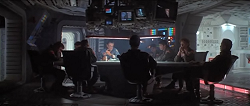
\includegraphics[width=\figwidth]{pics/8/2.png}
	\end{center}
\end{wrapfigure}
Both sides sit and glare at each other until the hooded figure observing the meeting clears his throat in a menacing way. 
Sarge gives Nubby, the squad’s quartermaster, a meaningful look. 
Muttering under his breath and moving with exaggerated slowness, Nubby pulls some exotic looking weapons from a storage case and lays them on the table. 
At a nudge from Sarge he also brings up two small crates, then sits back and nervously watches as a tall, thin man leans across the table and inspects them. 
After the thin man sits back down and has a short conversation with his team, Sarge gets to his feet. 
In a voice trembling a little with nerves, the noncom prepares to make what might be the most important deal of his life.

\greentext{>”We’ll offer these weapons, two crates of amasec, and will handle the combat training for the scribes, in exchange for your team taking ALL of the psykers.”}

\greentext{>The All Guardsmen Party: Good Soldiers, Bad Educators}


\begin{wrapfigure}{O}{\figwidth}
	\begin{center}
		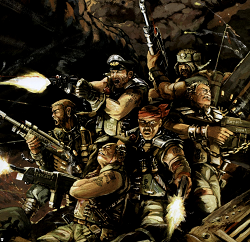
\includegraphics[width=\figwidth]{pics/8/3.png}
	\end{center}
\end{wrapfigure}
So no shit, there we were, on a ship headed out to some nameless Inquisition facility, to teach a bunch of fresh recruits how to be proper Inquisitorial goons. 
In our humble opinions this was stupid as hell: 
we were definitely goons, but it was hard to find anyone less proper than us.

When you hear the term “Agents of the Inquisition” you’d usually imagine a bunch of people in billowing cloaks, armed with masterwork power weapons, and acting all dark and mysterious. 
Maybe they’re not all beautiful or darkly handsome, but the ones that aren’t are definitely covered with impressive scars and fancy looking augmetics. 
You’d expect them to swoop in, interrogate and possibly torture anyone who looks shifty, maybe make a few other people disappear, then do something eldritch and fly away into the night. 
You would not expect a bunch of guardsmen wearing sweaty fatigues and constantly looking either bored, frustrated, or confused.

The point is that we didn’t look like proper agents, we didn’t act like proper agents, and we definitely didn’t have any idea how to teach a bunch of recruits to be proper agents. 


Sure all of our missions had been relatively successful, but aside from a few tactical situations we hadn’t actually done anything complex. 
We didn’t interrogate people, we didn’t assemble theories or hypotheses, and we didn’t leverage secret arcane knowledge. 
We just followed around our superior officer and did what we were told, if investigations were called for we typically just asked someone who looked smart to do it for us. 


All we really ever did was stand around until someone screwed up, then applied explosives and las-fire to the problem until it was fixed. 
While this seemed to work for us, it definitely wasn’t the way things were supposed to be done, and Oak probably wouldn’t thank us for teaching the rookies to act like that.

This was the worst idea since, well, putting Nubby in charge of buying a ship.

\begin{wrapfigure}{O}{\figwidth}
	\begin{center}
		
\includegraphics[width=\figwidth]{pics/8/4.png}
	\end{center}
\end{wrapfigure}
Okay, maybe it wasn’t THAT bad.

We weren’t handling all of these rookies’ education, just the final polishing. 
They’d already been through a few months of lessons on the basics of Inquisiting; 
some of Oak’s adepts had already taught them all that boring “what is chaos”, “where do tyranids come from”, and “why heresy is bad” stuff. 
They’d also supposedly been given a rundown of what their general role was and a few basic lessons on stuff like interrogation and disguises. 
We were expected to finish that training though; 
as experienced field agents we’d to be able to tell them what it was actually like to be on a mission and how to do their jobs correctly. 
Unfortunately, we didn’t even know what those jobs really were, much less how to do them.

Luckily, a second team of instructors had shipped out with us. 
They were all sleek and professional looking, and had experience in all those aspects of Inquisiting that we barely even understood. 
Ideally we’d have just handed off all the training to them, but there were too many students and too little time. 
Both of our teams would just have to split the load up as evenly as possible.

We were also accompanied by one of Oak’s personal Interrogators, a quiet fellow who liked to sit in corners and work on dataslates. 
The man didn’t actually seem very interested in our mission: 
he just gave us a basic briefing, handed over the files on the recruits, and then sat and worked on his slate while we hashed things out with the other team. 
Apparently the Interrogator’s job consisted of constantly organizing new groups of trainees, and he’d already started getting the next group together; 
which meant he really didn’t have any energy to spare on us. 
He was going to make sure we had a facility to train in and the right group of trainees, but as soon as we were in place he’d be flying off to set up the next batch, and the next, and the next. 
Once our classes got started, we wouldn’t see him until he showed up for the final review and shipped us all back to Oak.

\begin{wrapfigure}{O}{\figwidth}
	\begin{center}
		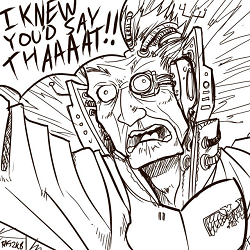
\includegraphics[width=\figwidth]{pics/8/5.png}
	\end{center}
\end{wrapfigure}
Aside from the initial briefing, our Interrogator probably said less than a hundred words to our team over the course of the trip. 
Some people would have been offended by this treatment, but we liked him; 
he seemed a lot less likely to get us all killed than any of our previous bosses.

Instead of bothering our Interrogator, we mostly interacted with the other team. 
They seemed like fairly solid folks, for a bunch of fancy agent types that is, but they were obviously a little unhappy about our presence on the mission. 
While they tried to be polite, it was easy to tell that they thought we were a bunch of dim grunts and didn’t believe any of our stories about our previous missions. 
Orders were orders though: 
if Oak said that we were half the training team then they’d make sure we did half the work. 


We would’ve settled for a quarter, or maybe an eighth.

Trainee records needed to be reviewed, locations needed to be chosen, resources needed to be requested, duties needed to be assigned, and lessons needed to be planned. 
As the only responsible members of the squad, Sarge and Doc handled most of this. 
Nubby was occasionally called in to lend a hand with the requisition paperwork, but Twitch and Cutter were left to their usual pastimes of paranoid booby trapping and obsessive sword drills 

Now, Sarge and Doc did their best to get us the cushiest jobs, but they were outnumbered and the other team wasn’t born yesterday. 
The crafty buggers weren’t about to let us stick them with all the crazies, criminals, and incompetents while we sat around drinking beers with a bunch of well trained PDF troopers and Arbites. 
In the end we all sat down to a negotiation and got the best deal we could.

At least we managed not to get stuck with the damned psykers.

\begin{wrapfigure}{O}{\figwidth}
	\begin{center}
		
\includegraphics[width=\figwidth]{pics/8/6.png}
	\end{center}
\end{wrapfigure}
Our squad would be in charge of four batches of trainees. 
There was a unit of PDF that had helped take down a minor daemon, and some violent priests who had burned out a few cults and were probably just being sent to us to get them out of the way. 
Then there was a group of criminals who were dumb enough to rob an Inquisition warehouse, but smart enough to talk their way out of an execution, and finally there were the scribes. 
Those damned scribes.

Not all scribes are useless little sissies. 
Hell, Cutter was a scribe. 
If he hadn’t been handed a chainsword during a pitched fight and subsequently discovered how much more fun being a raging berserker was, he’d probably still be pushing pencils and sorting files. 
In an extreme situation the meekest men and women can rise up and become heroes, surprising their enemies with berserk fury or vicious cleverness. 
Unfortunately when that heretic cult kidnapped a bunch of Administratum scribes and forced them to help translate a daemonic text, all the brave ones who fought their captors or sabotaged their translations were immediately killed. 


The scribes we got were the cowards, the weasels, the dimwits, and the bloody sheep; 
not a single one of them was even remotely qualified for any sort combat. 
Oak always needed more nerds for field duty though, and these scribes had enough mental fortitude to translate a chaos tome without going nuts. 
If we could make fighting men out of any of them he’d call it a win, even if the rest died in the process.

Both our squad and the other team could see what a shitshow training these bookworms to fight was going to be; 
no one wanted to trust them with a butter-knife, much less a firearm. 
It was obviously going to be bad, but all they needed was basic combat training and our squad could definitely provide that. 
So while the agents would handle all the assassins, infiltrators, cogboys, and psykers; 
we’d have the nerds, nuts, grunts, and scum.

\begin{wrapfigure}{O}{\figwidth}
	\begin{center}
		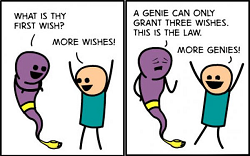
\includegraphics[width=\figwidth]{pics/8/7.png}
	\end{center}
\end{wrapfigure}
We touched down after a few weeks of idleness or frantic lesson planning, depending on whether you asked Twitch, Nubby, and Cutter or Sarge and Doc. 
The Interrogator directed both our squad and the other team to separate fliers, and said that the trainees and all our requested materiel would be waiting for us. 
As a sort of afterthought he reminded us that he’d be back in a few months for the final review, and then got back in the shuttle and left. 
It was reassuring to see that the other team was just as surprised and confused as us by his sudden departure.

Everyone stood there and milled around until the shuttle took off and a pair of men walked over from the parked fliers. 
They asked if there was anything else we needed to do here and reminded us that the trainees were waiting. 
As we split off to our flier, Sarge promised to keep in touch with the other team, who according to our guide, would be operating out of a separate facility half a continent away. 
This came as a surprise since none of us had paid that much attention to the location briefing. 
We’d expected to all be in the same facility and able to work together. 
Honestly it was all a bit distressing: 
our boss had just ditched us and the people we’d planned on asking for help and advice would be nowhere near us. 
We were going to be pretty much alone with the trainees. 
Sarge and Doc began to really worry about the quality of their plans, and the rest of us felt just a little guilty about slacking off.

Once we boarded the flier, our guide introduced himself as one of the Interrogator’s organizers. 
There were four of them at the facility: 
a doctor to watch the trainees’ health, a pair of tech-priests to keep the place running, and him. 
He was the facility administrator and would be getting everything ready for us. 
He’d handle all the paperwork, interface with the local authorities for us, and do his best to fulfill any supply requests we made. 
Twitch immediately asked for several tons of explosives, but Sarge interrupted the Administrator before he could finish asking what type.

\begin{wrapfigure}{O}{\figwidth}
	\begin{center}
		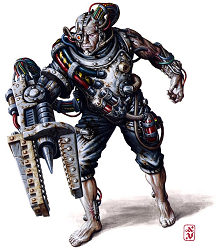
\includegraphics[width=\figwidth]{pics/8/8.png}
	\end{center}
\end{wrapfigure}
Sarge gave the Administrator a quick rundown of who in the squad was considered mentally fit, and what constituted a reasonable request. 
To his credit the man didn’t seem to be worried or confused by any of it, he’d probably worked with teams weirder than us. 
Hell, there was probably an all psyker team out there somewhere.

The planet we were flying over was reasonably pleasant looking. 
It seemed moderately developed world with no obvious specialization: 
there were a few large cities, a few small hives, a major manufactorum or two, and a fair bit of farming. 
A nice place with a breathable atmosphere and, at least where our base was located, a comfortable climate.

According to the Admin there weren’t any horrible political crises, religious schisms, genestealer cults, or major wars currently on the planet. 
He said there were occasional issues with feral orks, which made Twitch very unhappy, and of course there were always criminals and minor cults, but this was still the nicest planet we’d seen since enlisting.

The first thing we saw when we landed and the flier’s doors opened was a pair of big servitors bearing down on us. 
Twitch immediately opened fire and Cutter drew his sword and began to charge; 
luckily the rest of the squad intervened before any real harm was done. 
After Doc had explained our previous experience with servitors to a rather annoyed tech-priest, the Admin introduced to the rest of the base staff and we got settled in.

Doc went off with a scary looking doctor lady to look at medical records or something. 
Sarge got a base tour from the Admin and scheduled a morning review of the trainees. 
Twitch went off with the less annoyed of the two tech-priests to inspect the perimeter while Cutter and Nubby were left with the bags. 
After making sure both the cargo servitors and the tech-priest weren’t possessed, they loaded up our gear and went to get the squad’s quarters in order.

That night we got together, reviewed our lessons, and collectively panicked.

\begin{wrapfigure}{O}{\figwidth}
	\begin{center}
		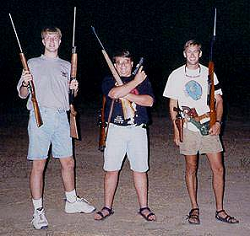
\includegraphics[width=\figwidth]{pics/8/9.png}
	\end{center}
\end{wrapfigure}
In the morning we marched onto the central training field looking imposing and professional in our Evil Goon Uniforms. 
Well, trying to at least. 
Sarge looked fine, but Doc looked like he was about to throw up, Twitch had spent all night messing with the perimeter defenses, no one had told Cutter to clean his uniform so it had a fair bit of blood on it, and Nubby looked like Nubby. 
We weren’t sure whether it was a good or bad thing that the trainees didn’t look any better.

Aside from the PDF, none of them were in matching uniforms; 
this offended our guardsmen sensibilities even before we even registered what the owners looked like. 
Their spastic collection of clothing included: 
priestly robes with hand sewn =][= symbols, poorly fitted bodygloves, ground-dragging trenchcoats, several sets of old and battered scribes’ robes, and to top it off, two of them had the poor taste to dress up like Cadet Commissars. 
They looked like idiots, they milled around on the field like idiots, and what they held in their hands proved they were idiots. 
Every, single, one of them was armed.

Not just armed, but heavily armed. 
Someone must have opened up a giant crate of autoguns, handcannons, and swords then told everyone to take whatever looked cool. 
One of the criminals looked like he was carrying over a dozen pistols, an old scribe was struggling to hold up a heavy stubber ,and some idiot had let all of the priests have hand flamers. 
As we stared at the mob of trainees, we realized that no one here had heard of trigger discipline and, judging by the flickering pilot lights on those flamers, they hadn’t heard of safeties either. 
Twitch and Nubby tried to casually move behind Sarge and Cutter.

Upon seeing such a shameful display, Sarge’s NCO instincts kicked in and he started bawling out the recruits. 
Unfortunately, before he could get up to speed there was a loud bang followed by a scream. 
The shouting had surprised one of the scribes and he’d shot himself in the foot.

\begin{wrapfigure}{O}{\figwidth}
	\begin{center}
		
\includegraphics[width=\figwidth]{pics/8/10.png}
	\end{center}
\end{wrapfigure}
While Doc hauled the idiot off the field we had a quick discussion then Sarge readdressed the trainees in a much quieter voice. 
After a brief introduction he ordered everyone to go store their weapons, unloaded and with their safeties on, then come back in an hour wearing proper exercise attire. 
As the mob dispersed Nubby grabbed one of the PDF troopers and asked him and his squadmates to oversee the weapon storage: 
two self inflicted gunshot wounds in a day would be a bit much.

Eventually everyone filed back onto the field, mostly disarmed and more appropriately dressed this time. 
It was tempting to start yelling at them about proper formation and posture, but we understood that those weren’t something an Inquisition agent needed, so we skipped over the drill sergeant routine. 
Sarge reintroduced us, explained what aspects of their training we’d be handling, and then went about splitting everyone into groups based on role and fitness.

The general plan was to split each day up between PT, weapons drill, lectures, and team exercises. 
In theory, everybody would be working together smoothly after a few weeks; 
then we could look into more complex exercises or getting in some outside experts to talk about stuff like cogitators and disguises. 
That plan fell apart before the first week was over.

\begin{wrapfigure}{O}{\figwidth}
	\begin{center}
		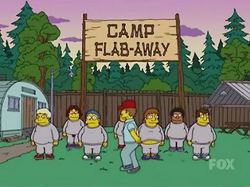
\includegraphics[width=\figwidth]{pics/8/11.png}
	\end{center}
\end{wrapfigure}
Every day started with physical training, but instead of Sarge leading everyone through their morning jerks together, they had to be split up. 
Sarge took the few healthy recruits and put them through the usual routine, Twitch did his best with the moderately unfit, and Doc handled the ones that looked like they were going to have a heart attack. 
This division slowed everything down a lot, and the problem was compounded by the difficulty of getting everyone out onto the field at a reasonable time for PT, which is to say before dawn. 
In the Guard, we would have just flipped them out of bed and dragged them to the field, but some of those scribes looked like they were at death’s door and we wanted to get as many as possible through the program.

As the days went on PT began to start later and later in the morning, and trainees started sneaking out of Sarge and Twitch’s classes. 
Aside from the PDF and a few scribes who seemed keen on their change of lifestyle, all the little buggers seemed bent on avoiding as much work as possible. 
If we didn’t keep an eye on them and send them back, then they would all wind up lazing around with Doc’s band of old fogies, asthmatics, and land-whales. 
Of course, avoiding hard work was a perfectly understandable goal, in fact most of us swore by it; 
but that sort of thinking was supposed to be reserved for proper guardsmen, not trainees. 


We spent a lot of time forcing the lazy bastards to work, and it didn’t endear us to them.

\begin{wrapfigure}{O}{\figwidth}
	\begin{center}
		
\includegraphics[width=\figwidth]{pics/8/12.png}
	\end{center}
\end{wrapfigure}
If anything, the weapons drills were going worse. 
Nubby and Cutter were working their asses off, but every damned recruit had a different weapon, and most of them had no clue how to use them. 
While standard Guard weapon drills can teach almost anyone to use a lasgun, they aren’t very good for explaining how to use a side-fed autogun, a bolt action anti-armor rifle, or a bloody crossbow. 
Nubby spent more time figuring out how to use each trainee’s random-ass weapon than teaching them how to actually shoot. 


Cutter wasn’t doing much better with the close quarters combat training. 
He couldn’t even blame the trainees random weapons, since after one of the scribes lost a finger during his first lesson, he’d confiscated everything and handed out wooden sticks. 
The problem was that everyone was either over excited or afraid of getting hit, also Cutter was just a really bad teacher and most of the scribes were terrified of him. 
He was terrible at pulling his blows, looked like he was genuinely trying to murder whoever he was practicing with, and really couldn’t explain how to properly use a weapon without demonstrating. 
At full speed. 
On a live target. 


The few trainees that weren’t scared shitless thought of Cutter as a complete simpleton, and generally ignored everything he said or wandered off at the first opportunity. 
Except the priests that is. 
Those damned priests took a shine to him, and seemed to think that his berserk fighting style was the best shit ever. 
Before we knew it we had a whole group of idiots who thought the best way to fight was by recklessly charging the nearest enemy. 
This had the side effect of making the scribes afraid of the priests.

We never got to the whole lecturing or group exercise part of the plan during the first week: 
the PT and drills just took too much time. 
There were over a dozen injuries that week, ranging from sprains to burns to gunshot wounds. 
Things were not going well, and the trainees’ morale was getting low.

\begin{wrapfigure}{O}{\figwidth}
	\begin{center}
		
\includegraphics[width=\figwidth]{pics/8/13.png}
	\end{center}
\end{wrapfigure}
The scribes were generally terrified and exhausted, and obviously thought of us as a bunch of dumb grunts that were only there to torment them. 
Most of them seemed sure that this was either some bureaucratic screwup or a pointless formality before they got cushy desk jobs. 
As time went on they got more and more snippy, and none of us could think of any way to deal with the problem without falling back on the Guard method, i.e. 
beating the shit out of anyone who complained. 
Unfortunately, Sarge and Doc vetoed this solution on the grounds that the Inquisition probably considered these scribes to be more valuable than the average Guard-trainee, and would frown on any breakage.

On top of this, the scum and priests were developing some worrying habits. 
The criminals were a relatively minor issue: 
they’d quickly figured out that we were usually too busy keeping the scribes in line to watch them, and were generally slacking off. 
They were staying out of the way, but their general contempt for us wasn’t doing our reputation any favors, and they persisted in antagonizing all the other recruits. 
At Doc’s suggestion, Nubby was put in charge of winning over his criminal brethren, and explaining the fine line between malingering and malicious lingering.

Meanwhile, the priests were developing that special flavor of crazy (mad zealotry with a dash of pyromania) that we recognized from every damned Inquisitorial cleric we’d worked with. 
They were far too eager for a chance to use their flamers on a live target for our liking, and the relationship between them and their less-than-holy fellows was getting rather strained. 
It was obviously only a matter of time before one of the priests snapped and tried to “purify” someone, but we weren’t exactly sure how to deal with the problem before it happened. 
Our attempts to convince them to “stop being crazy” and detailed explanations of what would happen if they lit anyone on fire without our direct orders were just met with blank stares and mutters that sounded like “damned is the sympathizer”.

Finally, and to our considerable surprise, the PDF were causing problems too. 
Most of them were solid troopers, and we’d have been happy to have them at our back any day of the week, but there were two damned Cadet Commissars mixed in with them, and they were NOT happy about taking orders from lowly guardsmen. 


\begin{wrapfigure}{O}{\figwidth}
	\begin{center}
		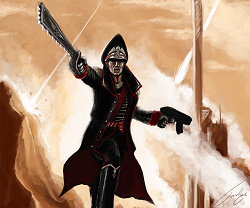
\includegraphics[width=\figwidth]{pics/8/14.png}
	\end{center}
\end{wrapfigure}
Those two Commissar wannabees screwed things up to no end. 
These weren’t the fun, happy, drink-and-play-cards-with-the-men Commissars, these were the ones with the whips. 
We knew their type, they had probably been itching for their final promotion so they could start performing field executions without asking permission first. 
Both of them probably soiled their pants in glee when they got a job offer from the Inquisition. 


Anyway, they were all set to start climbing the ladder towards becoming the scariest bastards in the Imperium, and then a bunch of lowly guardsmen came along and started bossing them around. 
They were not happy campers and neither were we.

Our problem was that, as guardsmen, we were bloody well programmed to fear and obey any Commissar we met, which made it damned hard to give them orders. 
Hell, it was all we could do not to salute them. 
Both of them performed well on the field and range, but they ignored most of our half-hearted orders and bossed around all the other recruits, especially the PDF troopers. 
Those poor buggers had apparently known the Commissars for a while and were absolutely terrified of them.

The end result was that our authority began to really suffer, and the trainees’ morale dropped even further. 
We made a few attempts to convince the Commissars to behave, but even appeals to the importance of proper discipline and troop morale, which was the whole purpose of Commissars in the first place, failed. 
They just knew, with absolute certainty, that they were better than us in every way and should have been in charge. 
Doc suggested transferring them to the other team, Nubby and Twitch were in favor of just shooting them, and Cutter actually liked them since they were good sparring partners. 
Sarge decided to give it a little longer and see if we couldn’t straighten them out.

\begin{wrapfigure}{O}{\figwidth}
	\begin{center}
		
\includegraphics[width=\figwidth]{pics/8/15.png}
	\end{center}
\end{wrapfigure}
Eventually we got the fitness regimen and weapon drills running smoothly enough for us to devote some time to lectures and team exercises. 
Neither of these went well.

Lectures don’t work well when the students don’t respect their teacher, or believe anything they say for that matter. 
When we talked about our previous missions they’d nitpick everything we said, analyzing every stupid decision we made, or pointing out all the things that couldn’t possibly have happened. 
Twitch got in a heated argument about whether a box full of Orks could possess a regiment of guardsmen, and Cutter decked one of the scribes after he kept pointing out that a Knarloc couldn’t survive in a spaceship. 
The priests would interrupt our stories with accusations of heresy, and those damned Commissars started riding our asses about not following standard procedures, especially the part where we didn’t purge the orky regiment. 
The only ones who didn’t cause problems were the scum and PDF troopers, but they seemed more interested in enjoying the stories than learning anything. 
Instead of serving as a demonstration of effective strategies, our evening storytimes turned into a sort of horrible, aggravating torture. 


The practical demonstrations went a bit better, but not much. 
While it was hard to argue about the truthfulness of a lecture on the planting and defusal of mines, the students tended to question why it would be their job to worry about that sort of thing when there’d be tech-priests around, or guardsmen for that matter. 
It was damned hard to get the little buggers to understand the importance of being a well rounded agent instead of a specialist, especially when they could point out that we were pretty damned specialized ourselves. 
They kept complaining that they were here to learn to be Inquisitorial investigators not guardsmen. 
Well, except the PDF troopers; 
they were fine with the idea of being guardsmen, bless their little olive-drab hearts.

\begin{wrapfigure}{O}{\figwidth}
	\begin{center}
		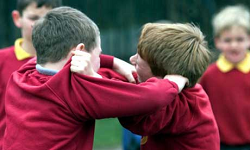
\includegraphics[width=\figwidth]{pics/8/16.png}
	\end{center}
\end{wrapfigure}
The team exercises were a complete fiasco. 
We worked damned hard with the Admin and his tech-priests to set up realistic combat scenarios, but the trainees seemed hell bent on ruining them. 
It wasn’t just that they kept on failing spectacularly, they also tended to interrupt things with pointless complaints about the exercise’s quality. 
It’s utterly infuriating to hear one of your recruits bitching about the “special effects” instead of properly covering their teammate.

Eventually we started leading the exercises ourselves, just to keep everyone moving. 
That stopped most of the complaining, but it’s much harder to fix stupid, so almost every run still ended in failure. 
The big problem was the Scribes, who had a tendency to trip over their feet and collapse from exhaustion. 
They weren’t much better when upright either: 
somehow they managed to shoot their teammates, and occasionally themselves, more often than their targets. 
It was amazing, if we’d used live rounds over half of the trainees them would have died; 
as it was the priests managed to torch an entire test area and badly burned a few of their fellows. 
It was enough to make a guardsman cry, but those test scenarios were nowhere near as bad as the competitive exercises.

Imagine a large group of children playing scrumball: 
the big ones knocking over the little ones, the mean ones ganging up on the meek ones, and the bossy ones ordering the other kids around. 
Now arm everyone.

There weren’t any deaths, but that was all you could really say for it. 
There were petty arguments over objectives, teams would frequently dissolve into in-fighting, there was no tactical coordination, and no matter who won each exercise, the scribes on both teams lost. 
Aside from the usual injuries there were two shankings, a few cases of “excessive whipping” and one of the clerics bit an ear off. 
Doc and the base surgeon managed to reattach it, but that scribe wasn’t ever going to look at priests the same way after that.

We were about ready to cave in and ask the other training team for help, when the Admin told us he’d spotted a nice milk run for our trainees. 
All of us were ecstatic, we figured a nice simple combat mission was just what was needed to straighten everyone out.

In a way we were right, the mission did result in a lot of straightening; 
just not in the way we thought.

\begin{wrapfigure}{O}{\figwidth}
	\begin{center}
		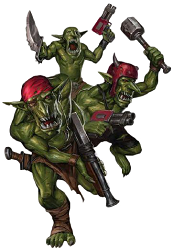
\includegraphics[width=\figwidth]{pics/8/17.png}
	\end{center}
\end{wrapfigure}
The Admin had a nice arrangement with the local government. 
A few of his contacts kept him apprised of any missions that could be used for training, and if the instructors accepted, the local forces would stand back and let the trainees have a crack at the problem. 
This was a pretty agreeable arrangement for all parties involved.

Now, we didn’t have any illusions about the quality of our trainees. 
They were utter shit, but this was the milkiest of milk runs. 
A feral ork raid had crawled out of a section of the swamps where they bred, sacked a few farms, and then ran back to their hovels with the loot. 
A fair sized counter-offensive was being formed by the locals to purge the nest, possibly with the help of the other team’s trainees, but we knew that was far out of our pathetic batch’s league. 
Instead, we had our eyes on one of the sacked farms, where a few straggling gretchin and squigs were still wandering around. 
Our trainees could fly in and have a nice simple game of Hunt The Gretchin, while we watched and made sure everyone stayed safe.

It was just about the easiest mission you could ask for. 
Hell, a grocery run in a lower-hive hab block was more dangerous. 
These were feral gretchin and completely ordinary squigs: 
they were weak, stupid, cowardly, and armed with nothing but knives and pointy sticks. 
Our trainees would be armed with high-quality ranged weapons and they could just slowly sweep the area, gunning down the little buggers before they even got close. 
We put together a clean and simple plan of attack, made sure everyone understood their role, and even checked their weapons for them. 


There was no way that anything could go wrong. 
The op was practically foolproof: 
we would have trusted it to a bunch of kids with slingshots. 


It was amazing how hard they screwed it up.

\begin{wrapfigure}{O}{\figwidth}
	\begin{center}
		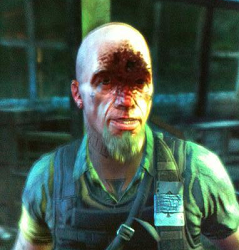
\includegraphics[width=\figwidth]{pics/8/18.png}
	\end{center}
\end{wrapfigure}
The locals had a cordon set up around the farm to keep the orkoids contained, and had given us a command tent to sit in while the trainees deployed. 
This meant we were a few hundred meters away when the screaming started, but from what we could piece together when the smoke settled it went something like this.

Squad three was advancing across the southern field when their gunner, the scribe who’d picked the heavy stubber, spotted a gretchin fighting with a squig in a nearby ditch. 
We heard him call in the sighting, and then both he and a squadmate opened fire. 
A few seconds later, they stopped firing and announced their intention to advance and “confirm the kill”. 
The heavy weapons scribe walked over to the gretchin and squig, but instead of just headshotting them both and moving on, he prodded them with the barrel of his stubber.

The squig jumped up and bit his ankle, causing the scribe to fall face first into the ditch. 
This in turn prompted the wounded gretchin to latch onto his head and start scratching and biting like only an angry gretchin can. 
The scribe leapt to his feet, flailing his arms and screaming over the open channel until his squadmate removed the gretchin. 
Unfortunately, said removal was performed using a hand-cannon, and while the gretchin was very thoroughly removed, so was most of the scribe’s head. 
Then, while the teamkiller panicked and tried to perform first aid on a headless corpse, a second, unnoticed gretchin seized the abandoned heavy stubber.

In the end there were seven deaths, four serious injuries, and three arrests.

\begin{wrapfigure}{O}{\figwidth}
	\begin{center}
		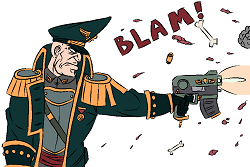
\includegraphics[width=\figwidth]{pics/8/19.png}
	\end{center}
\end{wrapfigure}
Of the seven deaths, only three were directly caused by the greenskins. 
The first was the teamkiller who was gunned down by the gretchin with the stubber. 
Another pair of gretchin accounted for a cleric who had a little too much faith in the Emperor’s protection and too little sense to run when his gun ran dry. 
The final one was a scribe who dove for cover in a mulch pit which was already occupied by a half-dozen squigs. 
As for the others: 
good ol’ fashioned friendly fire took down the poor PDF trooper who killed the gretchin with the stubber, as well as the scribe whose death started the whole mess. 
The last two deaths were Commissar related.

Most of the stubber-armed gretchin’s fire had been directed at squad five. 
The xenos’ poorly-aimed shots probably hadn’t come anywhere near actually hitting them, but the tracers flying overhead were enough to spook the two scribes in the squad. 
The two nerds ran for it, ignoring the orders and accusations of cowardice coming from the Cadet Commissar in charge of their squad. 
Enraged by this blatant cowardice and disregard for his authority, the Commissar drew his sidearm and placed three rounds through one of the scribes’ backs and drew a bead on the other. 
Before he could get the shot off though, a stray round, which neither the criminal or PDF trooper in his squad saw the source of, took him in the head. 
Someone stabbed his corpse a few times as well, but we put that down to a gretchin who must have somehow gotten hold of a ‘Type 7: 
Princeps’ Special’ switchblade.

As far as injuries went, the worst one was a cleric who got badly burned when he used his flamer inside an enclosed space; 
an enclosed space that just so happened to be made of wood and filled with hay. 
Aside from that, two trainees were badly hit by stray shots, and a scribe broke both his legs when he tried to take cover in what proved to be a very deep and very dry well. 
There were a few dozen lesser injuries spread across the whole group, but those were the only really nasty ones. 


All in all we lost eleven men, nearly a quarter of our trainees, but that wasn’t the end of it.

\begin{wrapfigure}{O}{\figwidth}
	\begin{center}
		
\includegraphics[width=\figwidth]{pics/8/20.png}
	\end{center}
\end{wrapfigure}
We’d provided all the trainees with comm-beads, figuring that good communications would help prevent screwups. 
None of us had thought to limit what frequencies they could transmit on.

One of the panicking scribes had decided the situation was FUBAR and called for backup. 
This by itself wasn’t a bad thing; 
hell, we were the ones who taught them to do it. 
Calling for help when shit got tough was a nice, sane reaction and we all endorsed it, but NOT over the emergency channel that everyone within fifty klicks was linked to.

As our squad mopped up the few surviving greenskins and Doc started triaging the wounded, the cavalry arrived. 
Several platoons of local PDF, a pair of chimeras, and a half-dozen fliers descended on the farm; 
all of them intent on rescuing our trainees from some sort of surprise attack by the Orks. 
We just barely managed to prevent another round of friendly-fire.

The reinforcements did help Doc treat the wounded and might have saved a few lives, but it was just about the most embarrassing moment in our careers. 
Sarge was vibrating between incandescent rage and horrible shame as he talked to officer after officer, thanking them for the help and assuring them the situation was under control. 
Doc kept himself busy with the wounded and avoided talking to anyone while Twitch and Cutter collected all the surviving trainees. 
Nubby just vanished; 
he tended to do that when people started asking awkward questions.

The cherry on top of everything was when another group of fliers landed and the other training team stepped out with their spiffy looking recruits in tow. 
They looked over the dead and wounded, asked a few of our trainees what had happened, then walked over to where Sarge was negotiating the release of three trainees who had attempted to appropriate a chimera and desert.

Words were had.

\begin{wrapfigure}{O}{\figwidth}
	\begin{center}
		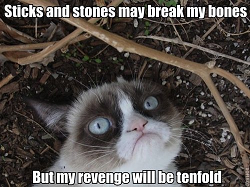
\includegraphics[width=\figwidth]{pics/8/21.png}
	\end{center}
\end{wrapfigure}
None of us were strangers to the odd reaming; 
it’s just part of being a guardsman. 
In a way, people yelling at you is almost comforting, it’s a reminder that the world hasn’t changed and you’re still right where you always were: 
at the bottom of the pile getting shit on by everyone else while you hold their asses up. 
Any of us could stoic our way through a dressing-down without blinking. 
This one crossed the line though.

It was one thing to be chewed out by your superiors, in private, for mistakes made by your and your men. 
It’s quite another to be berated by a group of your colleagues, in front of your subordinates and allies, for every damned screw-up since the Emperor decided that Horus would make a good warmaster. 
They even had the trainees chime in, whining about unfair treatment and poor lesson quality. 
That surviving Cadet Commissar was especially vocal, throwing out accusations of incompetence, cowardice, and heresy.

Sarge got the worst of it, being the nominal superior and first member of the squad they could find. 
The rest of us watched as he went from embarrassed to ashamed, to angry, back to ashamed, then straight past angry, furious, and murderous to a sort of zen state. 
The man was beyond anger, beyond shame and beyond fear; 
he was cold and calculating and was taking note of every single thing they said. 
The lecture petered to an end when the psyker on the other team started looking nervous and pulling at her teammates, suggesting that they still had a mission to do and they really ought to be going, right now.

As the other team got back into the gunships and flew away, Twitch asked if he should hit his detonators before they got out of range. 
Sarge just shook his head. 


We gathered everyone up and headed back to base. 
There was no talking during the flight or when we landed. 
No reprimands, no lectures, no punishments. 
Just directions to get some sleep.

That night we reevaluated our lesson plans. 
This would not happen again.

\begin{wrapfigure}{O}{\figwidth}
	\begin{center}
		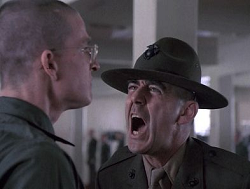
\includegraphics[width=\figwidth]{pics/8/22.png}
	\end{center}
\end{wrapfigure}
PT started an hour before dawn. 
Anyone who didn’t get up was dumped out of bed, tied by the leg to a servitor, and dragged out onto the field. 
There were no separate groups this time, everyone was doing the same drills we’d done as snot-nosed recruits. 
If you complained you got a licking from Sarge or Cutter and if you collapsed you got a stim shot from Doc or were left where you fell. 
If we thought you were malingering, Nubby would go over and give you a few good kicks (and ever since he got those augmetic legs, Nubby could really put the boot in).

Once the sun was good and up we led, or dragged, them all to the firing ranges where Twitch had laid out all of their weapons. 
Next to the rows of fancy firearms and melee weapons were several large crates which the Admin had busted his ass to get overnight. 
Sarge walked down the line of sweating trainees and asked each one to go get their weapons. 
When they went to pick up their autogun or flamer or crossbow, it was yanked out of their hands and they were given a battered lasgun and dull bayonet instead. 


This triggered a few complaints from the stupider recruits. 
They raised several points about the low quality of the weapons and their inexperience with them, and then tried to demand their old guns back. 
Sarge calmly explained that they were getting the lasguns because “Shut up and soldier, soldier”. 
Then he hit anyone who kept complaining.

They got the message pretty quickly and we outfitted everyone with a standard guardsman’s kit with optional toothless chainsword. 
Well, almost everyone: 
the remaining Cadet Commissar refused. 
He kept a death-grip on his weapons, and launched into a tirade about dignity and such, which ended with him being clubbed over the head by Cutter and dragged away by one of the servitors. 
That night we stripped him, wrapped him in duct tape and shipped him to the other training base with a note saying he had requested a transfer. 
He was not missed.

\begin{wrapfigure}{O}{\figwidth}
	\begin{center}
		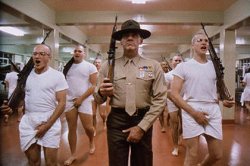
\includegraphics[width=\figwidth]{pics/8/23.png}
	\end{center}
\end{wrapfigure}
The next few days were nothing but PT and weapon drill. 
There were no team exercises, no demonstrations, and no lectures. 
Nothing but sweat, yelling, and as much food and sleep as they could get. 
No one was exempt; 
it didn’t matter if you were old or weak or overweight. 
The only way to get a break was to be too sick or injured to stand, and the second Doc or the base surgeon okayed it, you were back on the field. 


None of us knew how to be or train proper Inquisitorial Agents, but we damn well knew how to soldier. 
We were going to make every one of them into a guardsman, or kill them trying.

Once everyone began to adapt to the new regimen, we split them into squads and made the PDF troopers squad leaders. 
With both the Commissars gone the troopers really started to shine; 
every one of them proved to be a good leader and they were put in charge of keeping their squaddies in line and leading the drills. 
After all, they’d been through boot before and knew exactly how it should work.

With most of the basic training being handled by the troopers, we started doing demos and lectures again. 
This time we didn’t even try to fit our lessons to the trainees’ roles. 
Instead, we just focused on teaching what every guardsman should know and didn’t put up with any arguments. 
It didn’t matter whether or not it was something that an Inquisitorial Agent needed to know; 
we said it was important and they were going to learn it, whether they wanted to or not.

\begin{wrapfigure}{O}{\figwidth}
	\begin{center}
		
\includegraphics[width=\figwidth]{pics/8/24.png}
	\end{center}
\end{wrapfigure}
Twitch taught demolitions and defusal. 
He made sure every trainee knew how to plant explosives, set traps, put up alarms, and at least appreciated how tricky defusal was. 
He would rig realistic-looking and sounding explosives under their beds, and periodically send servitors to check their perimeter security in the middle of the night. 
None of the trainees liked him, but they learned fast.

Doc and Sarge made sure everyone knew standard Imperial Guard Combat doctrine, or at least the useful parts. 
Chances were they’d never need to know the correct way to call in an artillery strike or when to dig a foxhole, but it’d saved our lives in the past, so they were going to learn it. 
The field medicine lessons were a little more useful, and there were even some nice demos when the trainees hurt themselves. 
Doc practically glowed with pride the first time he got to demonstrate how to treat a lasgun wound on a whimpering priest.

Cutter mostly stuck to close quarters combat training, though he did throw in a few confusing lessons on the proper filing of Munitorum paperwork. 
There were still problems with the scribes being afraid of of him, but the PDF troopers were usually able to assist, generally by abusing the terrified scribe until they decided it was easier to face Cutter.

Nubby’s lectures were dedicated to scrounging, weapon maintenance, and how much criminality you could get away with. 
The shadier trainees found these lessons surprisingly educational and started warming up to the little bugger. 
The rest of us didn’t ask where they went on their field trips.

We all came together to teach our single most important class: 
Not Dying In the Inquisition. 
Now that we’d established a proper respectful atmosphere, our stories were much better received. 
We started slowly and laboriously going over every single battle we’d fought and every death we’d witnessed. 
We pointed out how explosives solved almost every problem, how psykers tended to ruin everything for everyone and often our problems were caused by our superiors. 
We crammed their heads with little pieces of common sense, each one backed up by horrible death or surprising victory, and made sure they could repeat each and every one back to us.

It might not have been the traditional Inquisition curriculum, but we hoped that none of our scribes would wind up reading random daemonic tomes and that our clerics wouldn’t die leading suicidal charges.

\begin{wrapfigure}{O}{\figwidth}
	\begin{center}
		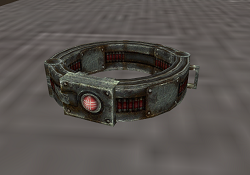
\includegraphics[width=\figwidth]{pics/8/25.png}
	\end{center}
\end{wrapfigure}
Of course, everything wasn’t magically better. 
Some of the trainees couldn’t take the strain and others tried to desert. 
We didn’t waste any time on frail ones: 
they were handed over to the Administrator in the hope that he’d find a place for them somewhere else. 
The deserters were retrieved and fitted with good ol’ fashioned penal legion collars for a few days while we explained how preferable death was to angering the bloody Inquisition. 
After that was fully explained, we removed the collars and offered them another chance to run. 
There were no takers.

Finally, there were also a few recruits who were just so abysmally bad with their weapons that we just gave up on them. 
There’s only so much you can do for someone who hits themselves more consistently than their target. 
Anyway, between the incompetents, the wounded, and the unfit, we lost another eight trainees before we started doing exercises again; 
but the ones who could hack it performed much better than they had before.

We ran them through the usual Guard training drills, complete with pig guts and razorwire. 
Everyone hated it and even the PDF troopers complained about the stupidity of learning trench warfare as an Inquisitorial agent, but they still went through the exercises and that’s all we cared about. 
We kept making the drills worse and worse, with Twitch adding dozens of little surprises, Doc and the base cogboys transforming servitors into horrible monstrosities, and Nubby bellowing horribly retarded orders at them while they drilled. 
They bitched, they moaned, and they began to really hate our guts, but that hatred was the final ingredient needed to really bring them together.

When we started the competitive exercises again they actually worked like teams. 
The scribes were still the weak link in most squads, but their squadmates and leaders began to actually work to support them instead of ignoring or mocking them. 
They were doing damned well, but we didn’t let them get overconfident: 
if a team was kicking too much ass, we’d enter the exercise ourselves and show them how it was really done.

\begin{wrapfigure}{O}{\figwidth}
	\begin{center}
		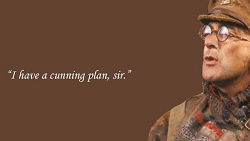
\includegraphics[width=\figwidth]{pics/8/26.png}
	\end{center}
\end{wrapfigure}
After a few months of grueling training, things were definitely starting to shape up and we began to think about other projects. 
None of us, except maybe Cutter, had forgotten the way the other team had lectured us in front of everyone. 
It might have been justified and we couldn’t deny that it had been what really kicked us into gear, but they’d crossed several lines and we felt a little revenge was called for. 
Nothing too bad mind you; 
after all, the training had to continue. 
Just enough to put them in their place and maybe boost our trainees’ morale a little.

Now anyone can hatch a revenge plot, but it takes a special type of person to come up with one that perfectly balances nefariousness, aggravation, embarrassment, and quasi-legality. 
Specifically, you need someone with a complete lack of scruples, a penchant for antagonizing behavior, and what might be called a Criminal Mind; 
which is to say someone like Nubby Nubbs. 
Of course we didn’t just let him plan it all himself, we’d learned THAT lesson, but he had a few very interesting ideas which served as the basis for our plot.

The Admin was asked to keep an eye out for a few things that might fit the bill, and before long we got lucky. 
A handful of carefully worded messages were sent, some palms were greased, and a few interesting rumors were started. 
Soon, both Inquisitorial training teams were informed that some mass disappearances were happening in the slums of one of the planet’s major cities. 


This was the perfect opportunity for the trainees to test their investigative skills! 
We suspended our drills, called in some fliers, and got the trainees disguised as harmless civilians, which is to say that we told them to leave their helmets behind and throw coats over their flak armor. 
Once their cunning disguises were in place, Sarge gathered everyone up and informed them of the situation. 
He explained what we’d heard and who we’d heard it from, and then asked them to remember the first rule of being a guardsman.

\begin{wrapfigure}{O}{\figwidth}
	\begin{center}
		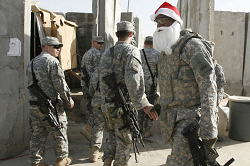
\includegraphics[width=\figwidth]{pics/8/27.png}
	\end{center}
\end{wrapfigure}
Of course, there are a few first rules of being a guardsman and there was a little confusion about which one Sarge meant. 
It wasn’t: 
“The gun is always loaded”, “Stay the fuck in cover”, or “If at first you don't succeed, call in an air-strike” and it DEFINITELY wasn’t: 
”It’s not stealing if they’re not from your unit and they didn’t really need it”. 
Nubby got a hard look from Sarge after that one.

With a weary sigh, Sarge explained that the First Rule of Being a Guardsman in the Inquisition is: 
“If the job looks hard, make sure you actually have to do it first”. 
None of the trainees seemed impressed with this piece of wisdom; 
at least, not until the rest of us volunteered some reasons why these disappearances might not be their problem. 
Then, because subtlety is completely overrated, we also suggested a few things that could be done with their time in the city if this turned out to be someone else’s problem. 
That got them thinking, and as everyone boarded the fliers, we heard the squad leaders talking. 
They were already brainstorming who they could dump this mess on, and what to do with their R\&R afterwards. 
Bless their weasley little hearts.

There was no point messing around with subtle entrances, we just landed at the largest police barricade, blatantly flashed our credentials, and turned things over to the trainees. 
We watched, tears in our eyes, as they practically marched onto the scene, looking exactly like a bunch of guardsmen trying unsuccessfully to look like civvies. 
They were growing up so fast.

The squads split up and stomped around the cordoned area with a complete lack of subtlety, loudly asking questions about whether there were any evil cults, daemons, or mutants around. 
If you knew where to look, you could see the other team’s cleverly disguised or concealed trainees staring with their mouths open. 
Within minutes, one of their instructors appeared out of the shadows, and asked us just what in the Emperor’s name we thought we were doing here.

\begin{wrapfigure}{O}{\figwidth}
	\begin{center}
		
\includegraphics[width=\figwidth]{pics/8/28.png}
	\end{center}
\end{wrapfigure}
While Sarge was the one the agent approached, the whole squad stepped back and let Nubby be the spokesman; 
it was just funnier that way.

The conversation was needlessly long and incredibly aggravating for the agent. 
It was hard as hell to keep a straight face as Nubby ignored accusations of incompetence and blatantly lied about our trainees’ expertise in tracking, interrogation, and “gen’ral investimagashun”. 
Eventually, the exasperated agent gave up on logic and tried bartering, prompting Sarge to step in and cut a deal. 
Our trainees were pretty much done here, so we’d go off and investimagate somewhere else in exchange for the other team agreeing to hold nightly meetings with us to discuss findings and progress. 
After all, if they were so much better than us, our trainees needed to see how it was done and maybe, just maybe, our boys would find something they didn’t.

That done, we marshaled the trainees up and left the area. 
Once everyone was back to the fliers, we handed operational control over to the squad leaders and adopted the role of observers. 
One of us tagged along with each group as they followed their leads, answering any questions they had, and occasionally making rather unsubtle suggestions.

That night everyone met up in a nice warehouse near the local PDF base. 
To our delight, one of the squads had attained it by simply asking nicely, and had split their day securing the perimeter and sneaking in naps. 
As the meeting time approached, a few of the other team’s trainers and trainees found their way in and provided com links to the members in the field. 
When everything was set up, Sarge shouted our troops into order, and suggested that both teams should take turns presenting the facts they’d gathered. 
The other training team’s leader agreed.

\begin{wrapfigure}{O}{\figwidth}
	\begin{center}
		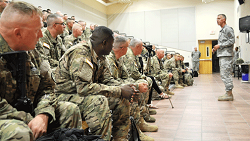
\includegraphics[width=\figwidth]{pics/8/29.png}
	\end{center}
\end{wrapfigure}
The agent explained that his trainees at the scene had found signs of struggle and a few emblems that matched no known cult, Imperial or otherwise. 
He talked a lot about footprints, dropped items, and other stuff that none of us listened to. 
When he wound down Sarge thanked him and asked Doc’s squad to present their findings.

The squad leader stepped forward and made his report in a nice clear parade ground voice. 
His team had gone to the local Arbites precinct and asked if they had seen any heretics, daemons, xenos, or mutants recently and if they knew any reason that groups of people would be disappearing. 
They had, of course, not seen anything, and had suggested looking for slavers or PDF recruiters as a cause of the disappearances. 
Sarge thanked the trainee, and turned the floor back over to the agent. 
Neither he nor his trainees seemed very impressed with the short report, but they didn’t make any comments and continued with their findings.

The other team’s trainees had tracked down a few witnesses and examined their minds and blah, blah, blah, no psychic activity, but definite signs of cults, blah, blah. 
Once he was done, Sarge’s team reported that none of the local temples had seen any xenos, daemons, or mutants, but the Church of the Divine Man and His Living Saints was pretty emphatic about the Third Convocation of the Emperor’s Blessing being a bunch of heretics. 
They had also suggested that the disappearances were a sign of imminent rapture, or that the Mechanicus was making an extra large batch of servitors.

By then, the agent was getting a little frustrated and had obviously noticed how little attention most of our trainees paid to his teams’ findings, though we were at least making sure none of them fell asleep. 
One of his trainees gave an exceedingly boring report about surveillance records and people wearing matching robes, which is, of course, a classic sign of cultists. 
Some of our trainees snickered at this.

\begin{wrapfigure}{O}{\figwidth}
	\begin{center}
		
\includegraphics[width=\figwidth]{pics/8/30.png}
	\end{center}
\end{wrapfigure}
Twitch’s team had chatted with the local PDF before securing the warehouse we were in and verified that they hadn’t seen anything weird. 
The PDF had also implied that maybe all of the disappearing people had just suddenly decided to move to a different city and it probably wasn’t anything sinister. 
At this point the agent and his trainees began to raise objections about the quality of our investigation. 
They seemed to think that all we were doing was asking random people if anything was wrong then just accepting whatever they said. 
None of us saw anything wrong with this though, so we just ignored their objections until they got on with their own reports.

Another batch of the other team’s trainees had done some snooping in the sewers and a few underworld establishments with mixed success, but those that weren’t waylaid by gangers had, of course, found more evidence of cultist activity. 
A short argument was triggered by a nameless wise-ass in the audience pointing out that the agent and his trainees could probably find evidence of cultist activity in their breakfast cereal. 


The mood was not improved by Nubby’s team’s helpfully confirming a sighting of one of the other trainees being worked over with a pipe-wrench in an alley. 
They had thought about intervening but didn’t want to blow the man’s cover, so instead they asked the wrench-wielder for directions to a notorious local bar and left the trainee to his super-secret mission. 
After that, they visited several local underworld leaders, verified that they hadn’t seen anything fishy or perpetrated any mass kidnappings, and politely asked them not to actually kill anyone until the investigation was over. 
The criminals had suggested the disappearances might have been caused by a press-ganging band from a navy or merchant vessel. 
On the way out, they had spotted the battered trainee lying in a trash pile, and had generously paid a few children to drag him to a public medicae.

The agent was starting to turn a funny shade of red now and the report from Cutter’s team was the final straw. 
They had gone to the local Administratum headquarters, but couldn’t get an appointment until tomorrow, and had decided to just call it a day.

\begin{wrapfigure}{O}{\figwidth}
	\begin{center}
		
\includegraphics[width=\figwidth]{pics/8/31.png}
	\end{center}
\end{wrapfigure}
All of us were accused of horrible incompetence, astounding laziness, and quite a few other things. 
We bore these accusations like the stoic guardsmen we were, but some of the trainees felt the need to respond by accusing the agent and his trainees of ridiculous paranoia. 
Sarge quieted them down and reminded them that paranoia wasn’t always a bad thing and pointed out how often Twitch’s had saved our lives. 
Being compared to Twitch did nothing to improve the agent’s mood and he stormed out with his trainees in tow.

As he left, Doc ran out after him and apologised for our behavior and lack of useful findings. 
This might have mollified the agent, but Doc followed it with an assurance that everything would be sorted out when we got our appointment with the Administratum. 
Once they were gone, everyone broke into laughter.

Our trainees weren’t stupid and they’d realized that we were playing with a stacked deck long ago. 
It had become a game: 
the stupider they thought we were and the more time they spent chasing imaginary cultists, the funnier it would be when we proved them wrong. 
We went to sleep proud of our trainees; 
they were adopting the proper cynical guard outlook surprisingly fast.

In the morning, we all went down to the Administratum for the meeting. 
Most of the trainees were left outside, but Cutter’s squad went in and we sat and watched as they went through the questions. 
The head scribe assured the squad that there were no heretics, daemons, or xenos around and only a small number of minor mutants according to the last census. 
As far as the disappearances went, they didn’t know anything about slavers, and neither the PDF nor Mechanicus had filed for a recruitment sweep. 
However, a Rogue Trader with a permit to press-gang had been cleared to operate in that area, and now that the scribe looked at it, there’d been a bit of bureaucratic mix-up. 
Apparently, a key piece of paperwork had been misfiled during press-ganging application process, and the local authorities hadn’t been properly informed.

\begin{wrapfigure}{O}{\figwidth}
	\begin{center}
		
\includegraphics[width=\figwidth]{pics/8/32.png}
	\end{center}
\end{wrapfigure}
So it was all just a misunderstanding, imagine that! 
Someone just needed to go get the press-ganging crew to fill out the paperwork again, as well as deliver a new batch of identification badges to them, since they’d somehow been issued some sort of decorative novelty pins covered with squiggly lines instead of the proper ones. 
To the apologetic head scribe’s delight, and without any prompting from us, our trainees immediately volunteered to go get the papers signed and deliver the proper badges. 
After all, it was their duty to get this mess sorted out as soon as possible.

A few hours later, we were all drinking and laughing in the rather nice hotel which the leader of the press-gangers was staying at. 
The man was very apologetic once we’d explained all the trouble that had been caused by the little mix-up. 
He promised to make sure his paperwork was properly filed in the future and invited us to have a few drinks in the hotel restaurant on him. 
A message was sent to the other team telling them we’d solved the whole mystery and recommending they head home, and then we let the trainees off the leash and had a nice chat with the press-ganger while we waited.

It took a while before someone on the other team came over to see what the hell our message was about, but none of us minded. 
When the sneaky looking trainee poked his head into the restaurant, he saw all of our students having a pretty wild party while our squad sat like kings at feast. 
Cutter grabbed the little bugger the second we saw him, dragged him up to our table, and prompted the rather tipsy press-ganger to explain the situation while Nubby filled in the drink-induced blanks. 
The look on that trainee’s face was priceless, and we all snickered into our beers as he scurried away to call his bosses.

A short while later, the whole other training team was standing in front of us, in the middle of a party that was off several types of hooks, glaring at us like we’d kicked their mothers and slept with their pets. 
Or vice versa; 
there was just a little bit of drinking going on.

\begin{wrapfigure}{O}{\figwidth}
	\begin{center}
		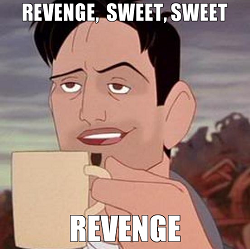
\includegraphics[width=\figwidth]{pics/8/33.png}
	\end{center}
\end{wrapfigure}
The other team didn’t believe us at first. 
Hell, we wouldn’t have believed us: 
it all looked too cut and dried, but there was more than enough proof. 
We had the official documents and permits, the logs from the shuttle that’d taken the civies away to their new and exciting lives aboard the Trader’s vessel, the note from the head scribe explaining the accident, and the press-ganger himself beerily waving and confirming that it was all him. 
There were no cults, no secret societies, and no complex cover-ups; 
well, at least there weren’t any involved in the disappearances. 
It was all just bureaucratic mix-up, a simple mistake. 
Just. 
Like. 
We. 
Said. 
It. 
Was.

It was glorious watching their faces as it sank in, seeing them go from disbelief to anger to utter disgust. 
We didn’t gloat too much; 
there’s such a thing as winning gracefully, but some of the inebriated trainees were a little less restrained. 
They might have made some very unpleasant enemies if the party’s designated thinkers hadn’t hauled them away in time.

Once everything had sunk in and we considered the score suitably evened, we invited the other team to stay and party with us, but they made lame excuses about needing to go see to their own trainees. 
As they left, their leader, the suave agent fellow, swore that they had actually found a cult, even if it wasn’t linked to the disappearances. 
Sarge told them to have fun and asked them to give us a call if they needed some fire support when they located the heretics or whatever: 
now that our point was made, we were done pretending to be even slightly interested in investigations. 


Our guests dealt with, we got down to the very serious business of teaching our trainees how to hold a proper victory celebration. 
Super-professional Inquisitorial educators, that’s us.

\begin{wrapfigure}{O}{\figwidth}
	\begin{center}
		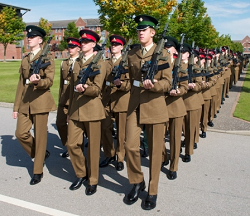
\includegraphics[width=\figwidth]{pics/8/34.png}
	\end{center}
\end{wrapfigure}
After everyone had slept it off, we cleared up the last loose ends and headed back to base. 
There was still a lot of training to do.

In our opinion, we’d made proper trainee guardsmen out of the lot and it was time to start polishing. 
We began to work heavy weapons and explosive drills into the schedule along with a few more specialized classes for the scribes and priests. 
We had the base staff act as guest lecturers, talking about more or less anything that was nerdy and Inquisition related. 
None of them were teachers really, or veteran field agents, but they knew a few things and passed them on to our nerdier recruits while we taught the others how to use missile launchers and heavy stubbers.

We tried to fill the remaining gaps by dumping piles of semi-restricted books and vids on the trainees. 
Lots of journals written by Inquisitors, after action reports, and other stuff like that. 
Honestly, we just had the Admin grab some of everything and let the trainees work it out for themselves. 
We certainly weren’t going to read all that shit; 
except for Doc that is. 
He tried to get us to read this book about longing for balls by some famous old crippled Inquisitor, but it was way too long and sounded like the diary of a perverted shut-in, so none of us could be bothered. 
He was a bit sore about that, but he got some sort of book club going with the trainees so it all worked out.

Everything was shaping up nicely as we got near the scheduled end of our training. 
Sure, we were down to thirty recruits from our original fifty, but we were reasonably happy with what we had: 
every one of them was a soldier now. 
Maybe a nerdier, scummier, or holier soldier than usual, but still a soldier first and foremost. 
Admittedly Oak hadn’t asked for a bunch of mudfeet, but if he wanted something else, he shouldn’t have put us in charge.

We were feeling pretty good about how everything had turned out. 
Then we got the call from the other team.

\begin{wrapfigure}{O}{\figwidth}
	\begin{center}
		
\includegraphics[width=\figwidth]{pics/8/35.png}
	\end{center}
\end{wrapfigure}
While we’d been doing our final polishing, the second team had been chasing the cultists they had spotted during the mission. 
Despite the shit we had given them about paranoia, they were a veteran Inquisitorial team, and if they still thought there was a real cult around here there probably was. 
We weren’t going to go look for it ourselves of course, we probably wouldn’t be very helpful and they certainly didn’t want us there, but the Admin had kept us updated on their progress.

The second team rebased, infiltrated, called in some local support, rebased again, and so on. 
It was interesting to watch them bouncing around the planet hot on the trail of something, and we made sure our recruits saw their progress: 
it was probably educational. 
Whatever they were chasing was serious: 
a few of their trainees died and someone or something messed up their psyker chick real bad. 
That didn’t stop them though, and eventually they found what appeared to be the cult’s primary evil lair.

We’d received a few little summaries about what they were dealing with. 
The cult was some sort of end of the world thing: 
worshiping ancient death gods, prophesizing their return, and other such silliness. 
As far as practical details went: 
everyone in the cult appeared to be suicidally devoted to it, and their base showed signs of some sort of weird archeo or xeno tech, but at least their doctrine was decidedly anti-daemon and psyker. 
While that last part was unquestionably good news, we found it a little unusual as well, since all the cultists we’d encountered were all about the warp-stuff. 
Also, something had mentally mangled the psyker chick, which didn’t track well with their supposed lack of warpy powers.

The cultists’ base didn’t look too huge or well armed, but it was a very weird cult so the other team wanted the purge done by someone more experienced with spooky stuff than the locals. 
Ideally they’d put out a call for reinforcements from Oak or some other Inquisitor, and then sit tight and observe the cult while waiting for backup to arrive. 
Unfortunately, something or other had lead them to believe that time was critical, so they were going to have to settle for us guardsmen and our dubiously-educated trainees.

\begin{wrapfigure}{O}{\figwidth}
	\begin{center}
		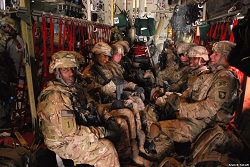
\includegraphics[width=\figwidth]{pics/8/36.png}
	\end{center}
\end{wrapfigure}
It was actually pretty exciting to get the call. 
Normally we liked to avoid things like angry cultists trying to kill us or being sent to storm a fortified position, but this was a perfect chance for our trainees to prove themselves. 
We were going to rip through those cultists like a chainsword through butter, or flesh, bone, and most types of metal for that matter.

Fliers came to get us, and we loaded up with a bit of everything. 
We figured that since no one was sure what was in the base, it wouldn’t hurt to be over-prepared. 
Between the standard gear, the specialist munitions our trainees knew how to use, and our own personal arsenal, we were ready for anything up to a titan. 
Of course Twitch pointed out that the base was just large enough to hold a titan, but we really couldn’t fit any more ordinance into the fliers.

The recruits were briefed, weapons were checked, and we headed out. 
As we flew, Sarge worried in his usual grumpy way and double checked the brief, Cutter made sure his chainsword was all greased up, and Doc wrote a soppy letter, just in case. 
Twitch was arguing with Nubby about how many detpacks it would take to cripple a titan while the little man tried to out-cheat a few trainees at cards. 
The recruits fidgeted in their seats and chatted with each other, displaying the usual first-deployment mix of nerves and excitement. 
We proudly noted that their excitement definitely outweighed their nervousness; 
they’d trained for this and were pretty confident in their skills.

We were about twenty minutes from our destination, flying low and slow, when something flashed out of the sky. 
It was directly ahead of us and came straight down, trailing fire at well over terminal velocity. 
It looked like a macrocannon shot, it sounded like a macrocannon shot, but it wasn’t part of a barrage and Twitch claimed the shock-wave that hit us wasn’t nearly big enough. 
We weren’t sure what it was, and it had struck right in the middle of the cult’s base.

The other team voxed and said they were moving in without us, just in case it turned out to be some sort of weird world ending shit. 
Sarge told the pilots to forget stealth and floor it.

\begin{wrapfigure}{O}{\figwidth}
	\begin{center}
		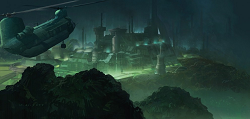
\includegraphics[width=\figwidth]{pics/8/37.png}
	\end{center}
\end{wrapfigure}
So no shit there we were, flying towards a cultist base that had just been cratered by a UFO, listening to the other team advance and hoping against hope that this wasn’t about to turn into a rescue mission. 


We made it almost all the way there before the screaming started.

A crude plan was formed as we landed. 
The other team had activated their locator-beacon and we were going to head right for it. 
Twitch would take a squad and secure the perimeter and fliers, Cutter would be on point with another squad, Doc’s squad would cover our rear, and Sarge would lead the rest of the squads from the middle with Nubby acting as aide. 
Nubby complained about the arrangement and was reminded that, after the whole ship-purchasing fiasco, he was banned from command until the Emperor stepped down from his throne and told Sarge otherwise.

The frequencies the other team had been using were a complete mess, filled with a few screams and lots of static. 
Something in here was screwing with comm signals, and their fancy low profile models weren’t punching through well. 
Ours were doing a bit better, but only the vox-casters were getting through clearly. 
One of the recruits with a caster was put in charge of cycling through their frequencies and telling everyone to fall back to our positions. 


The cult’s base was a sort of giant low bunker. 
It had one large entrance, a few side doors which we left to Twitch, and a huge-ass hole in the roof that was probably not in the original design. 
The hole was slightly on fire and appeared to be glowing green, so we decided to go in through the front door.

There was a trainee from the other team lying in a few pieces just outside the main entrance and the first cultist we saw was in similar shape. 
The second, third, and fourth cultists we ran into were all alive though. 
They were also nuttier than squirrel shit and armed with an automatic shotguns.

\begin{wrapfigure}{O}{\figwidth}
	\begin{center}
		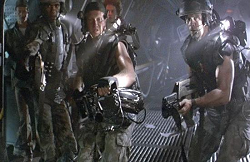
\includegraphics[width=\figwidth]{pics/8/38.png}
	\end{center}
\end{wrapfigure}
Luckily Cutter’s boys were pretty quick, only one was injured before a few grenades solved the cultist problem. 
After that scare we slowed down a little, there was no point in getting killed before we managed to rescue anyone.

The recruits put their breach and clear training to good use, room after room was flashed and secured as our force headed deeper into the bunker. 
We ran into a few more cultists and a lot more corpses on our way, and while we didn’t have any trouble with the hostiles, the bodies were a bit worrying. 
Some of the corpses had normal gunshot wounds, others had been sliced up by something very sharp, like a mono or force sword, and a few didn’t have a mark on them. 
Something here had been killing both friendlies and cultists, and was being damned weird about it. 
Nubby put his money on a daemonhost and began telling everyone about how he’d killed the last one we faced until the rest of us told him to shut up.

Things started to get bad after we found the main stair shaft for the bunker. 
Sarge left a squad to secure it, figuring that it was about the most important access point around. 
A few minutes after our main force left them, the squad lead voxed us and reported a man missing. 
Shortly after that, we heard las-fire and his second reported one man dead and two missing, including the squad lead.

A halt was called. 
Sarge told the cut-off squad to pull together and hold position, and then sent Doc and Nubby with a patrol to recover the squad before they were all picked off. 
Doc’s rescue-team didn’t run into anything as they backtracked, and when they arrived the squad was still intact, if badly shaken. 
A quick sweep turned up the two missing recruits dead in corners without a mark on them and the squad lead hacked to pieces. 


It was obvious that whatever had been hunting the other team and the cultists was stalking us now. 
Sarge mandated minimum groups of three, called Doc and the recruits back to the main force, and resumed the advance.

\begin{wrapfigure}{O}{\figwidth}
	\begin{center}
		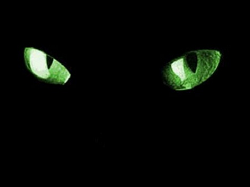
\includegraphics[width=\figwidth]{pics/8/39.png}
	\end{center}
\end{wrapfigure}
The recruits on our flanks began to report possible enemy contact, usually flashes of movement or odd sounds on their comms. 
During a brief firefight with a nest of cultists holed up in some sort of storage room one of our men dodged into a closet and didn’t come back out; 
he was dead by the time his squadmates noticed his absence and went to check on him. 
Two more trainees died this way, and a pair of recruits chased a fleeing enemy around a corner, only to find the cultist eviscerated and still twitching. 
They swore something had flashed away into a dark corner as they approached, but didn’t find anything when they checked.

Everyone was getting jumpy, and a trigger happy recruit nearly shot the first friendly we ran into. 
A few surviving trainees from the other team, usually in groups of two or three, followed our vox casters’ signal and made contact as we advanced. 
For the most part they were in good condition, if disorganized. 
Their command structure had fallen apart when their comms went down, and they’d been wandering around killing cultists until we’d shown up. 
Sarge put them on the flanks to act as scouts since they were stealthier than our boys, not to mention a little more expendable.

None of the rescued trainees had any useful info for us until we found a solo one with a nasty face wound. 
She was panicking hard and waving a power sword around in the middle of a brightly lit room, and 
it took both a tranq and a stimm from Doc to get her talking properly. 
Most of what the terrified trainee had to say was gibberish, but she was fairly insistent about glowing eyes watching from the shadows and blades coming through the walls.

The panicked trainee’s info fit with what we’d observed, and some of our former scribes said they recalled reports of daemons and daemonhosts phasing through solid objects or emerging from shadows. 
Most of us found this explanation for the attacks to be extremely worrying, but Nubby chose to look on the bright side, and began gloating about how he was always right and how much money everyone owed him. 
Sarge adjusted his standing orders to include staying away from walls and unlit areas, and then told Nubby to shut up and do something useful, such as figuring out a way to trap or kill whatever was stalking us.

\begin{wrapfigure}{O}{\figwidth}
	\begin{center}
		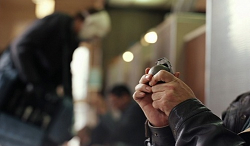
\includegraphics[width=\figwidth]{pics/8/40.png}
	\end{center}
\end{wrapfigure}
Nubby being Nubby, he immediately voxed Twitch, and dumped the problem on the demolitions trooper, while he assumed an “advisory role”. 
That’s not to say that Nubby didn’t do any of the work: 
someone had to accurately relay what materials were available, remind Twitch that nuking the temple from orbit wasn’t an option, and either take credit or assign blame depending on how the plan worked out. 
Anyway, between them they came up with a rather cruel, but surprisingly effective, solution.

At their request we began capturing a few cultists instead of killing them all. 
Nubby, with far too much enthusiasm, would tie them up, tape a short fuse grenade into their hands and pull the pin. 
Of course a few immediately let go of the lever and blew themselves all over the room we left them in, but most held tight. 
As the advance continued we heard the occasional explosion behind us, prompting Nubby to cackle and Doc to complain that this was probably not something we should be teaching the trainees. 
The traps worked though: 
two of the explosions resulted in odd high pitched screaming sounds and we stopped seeing the flashes of movement. 


While Nubby was fooling around at the rear, Cutter’s squad was starting to run ragged after so much time at the front. 
They’d taken the most casualties from the cultists and Cutter himself had taken a few minor wounds himself, so Sarge rotated them off the front and led the final push towards the other team’s beacon. 
As our force got closer, everyone began to hear the sounds of a firefight, and shortly after that we encountered the largest group of cultists yet.

The cultists were trying to force their way into a large room and failing miserably. 
We took up positions, counted down, and at Sarge’s signal our boys hit them in the rear with a few grenades and a whole lot of las-fire. 
For once, the attack went just about perfectly, and we mopped the cultists up with only a few minor injuries on the part of our trainees. 
Once the last injured cultist had been executed, we rallied together and carefully made contact with the what was left of the second team.

As we entered the room and automatically scanned it for threats, our attention was immediately grabbed by a massive hole in the far wall which opened into the bottom of the crater. 
We couldn’t help but notice that the everyone in the room had positioned themselves to cover it, as opposed to the door which the cultists had been attacking through. 
That did not bode well.

\begin{wrapfigure}{O}{\figwidth}
	\begin{center}
		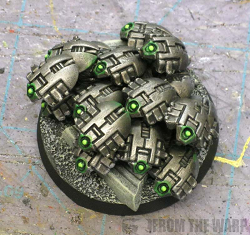
\includegraphics[width=\figwidth]{pics/8/41.png}
	\end{center}
\end{wrapfigure}
Not counting the handful we’d recovered on our way, the second team was down to just a dozen men and women led by the agent and cogboy instructors. 
Only the combat-focused trainees were left: 
there were a few former arbites, a pair of psykers, a handful of their more well-armed generic agent types, and that damned cadet commissar we’d “transferred” to them. 
They looked absolutely exhausted, and most of them were wounded to some degree, but they all perked up as we entered the room. 
Except for the commissar that is, he just glared at us.

The boss-agent gave us a quick rundown as we got our boys into position alongside his trainees. 
Apparently, when the UFO had cratered, his team had gone in fast and hard. 
A few of them stuck together to check out what had landed, but most had split off solo or in small groups to cover more ground or something stupid like that. 
They’d been kicking ass right up until they’d reached this room and poked their noses into the crater. 


The agent explained that the second one of his trainees had entered the crash site, everyone’s comms had gone down, the solo trainees started getting picked off, and his main force had been attacked by the ship’s defenders. 
Sarge was in the middle of asking what he meant by “ship”, when one of the men watching the crater shouted a warning.

Black and green metallic critters began boiling out of the crater-hole and everyone started shooting. 
The attackers were small, quick, and there was a whole lot of them. 
If it weren’t for the choke point between the room and the crater, we would’ve been in serious trouble: 
those things would’ve been a nightmare to face in an unrestricted area or close quarters. 
As it was, we were able to hold the tide of metallic attackers back with volleys of fire and a few grenades; 
at least until something covered with claws came out of the damned floor and shredded two recruits.

\begin{wrapfigure}{O}{\figwidth}
	\begin{center}
		
\includegraphics[width=\figwidth]{pics/8/42.png}
	\end{center}
\end{wrapfigure}
The situation started to go bad very quickly. 
The thing that had risen out of the floor was some sort of big metal spider-worm with scythes for arms; 
it positively screamed “close quarters combat specialist” and it was behind our main firing line. 


Now a proper guardsman can handle just about anything, but we prefer to fight our enemies from the maximum effective range of our current weapon or, better yet, the maximum effective range of the nearest artillery battery. 
The spider-worm was far too close for comfort, and it tore three trainees apart before it ran into one who could put up a real fight in melee. 
Even after its killing spree had been interrupted though, the thing’s mere presence played hell with our defense of the crater entrance: 
the fire keeping back the tide of metal bugs began to fade as recruits scrambled to safety or switched targets to focus on the new threat.

We managed to hold, but only just barely. 
Sarge barked the recruits back into position as our squad worked to personally deal with the spider-worm. 
Cutter led the attack with the commissar and agent-instructor backing him up in melee, while the rest of us fanned out and hit the thing with our heavier las-guns. 
It was not an easy fight. 
The enemy was tough, fast, and attacks had a disturbing tendency to pass through it; 
half the battle was just trying to line up attacks so they didn’t hit an ally on the other side if the thing phased out. 
To be honest Cutter didn’t really bother with that, he just depended on everyone else getting out of the way.

Whatever the spider-worm’s claws were made of, it was a nightmare to defend against. 
The metallic creature’s attacks sliced through armor like wet paper and just phased through any attempts at parrying. 
Only some incredible dodges kept Cutter and our close-quarters fighters alive long enough for us to figure out how to reliably hit the damned thing. 
It turned out that the trick was to wait for the exact moment it struck, and then hit it with everything we had while it was temporarily solid. 
Unfortunately, this strategy required someone to very nearly take a hit for us to launch our attack, but Cutter was more than willing. 
A few well timed volleys and a couple near death experiences later, the spider-worm collapsed in a sparking heap.

\begin{wrapfigure}{O}{\figwidth}
	\begin{center}
		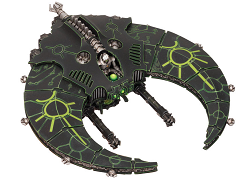
\includegraphics[width=\figwidth]{pics/8/43.png}
	\end{center}
\end{wrapfigure}
Sarge and Nubby took stock of the situation while Cutter ignored both Doc and the cogboy’s protests and wildly chopped at the remains of the spider-worm. 
A few trainees from both groups had died during the attack, mostly to the spider-worm, but a few of the smaller metal bugs had gotten through and done some unpleasant things before they were smashed. 
Ammo was getting low and we had a fair number of wounded, including Cutter, who finally collapsed after reducing what the cogboy called a “technological marvel” to a pile of scrap metal.

A quick council of war was held and the other team finished filling us in. 
They believed that the hostiles were a type of xenos called Necrons, and that the thing in the crater was one of their ships. 
Despite our general lack of proper Inquisitorial education, the name rang a faint bell; 
something about techno-magical powers, looking like skeletons, and refusing to die. 
That didn’t seem quite right to us, since none of the enemies we’d fought had looked anything like skeletons and the spider-worm seemed pretty damned dead now that Cutter was finished with it, but the agent and cogboy seemed fairly certain, so we just went with it.

Anyway, the ship in the crater was in surprisingly good condition, especially considering how it had arrived, which excited our better-educated counterparts to no end. 
They said it was both an amazing opportunity for Inquisitional research and a dire threat to the planet. 
Apparently, Necrons were famous for their use of teleportation technology, which was rumored to have the range and power to bring in an entire army of ground-troops from across the galaxy. 
Obtaining working samples of said tech for study was absurdly difficult, to say the least. 


So the agent and the cogboy were all excited about a chance to loot the ship, but we were a little more concerned about the whole “providing a gateway for an invading xenos army” aspect of things. 
Our well-honed survival instincts were telling us to call the locals and have them bomb the entire temple until the ship was either blown to pieces or buried under a few thousand tons of rubble, and then bomb it some more, just to be sure. 


The other team objected to this perfectly reasonable solution on the grounds that the Inquisition would consider an INTACT sample of Necron teleportation tech to be far more valuable than a mere planet. 
Unfortunately, they were able to back that incredibly stupid argument up with a less-stupid one about how the Necrons might start teleporting in before the locals got their shit together. 
Lacking any reasonable counter-arguments to that, we reluctantly agreed to head in and see if we couldn’t deactivate the ship’s teleporter-thingy. 
Twitch was commed, and we started getting ready for one hell of a breaching operation.

\begin{wrapfigure}{O}{\figwidth}
	\begin{center}
		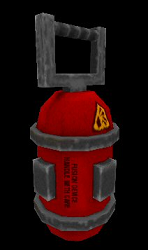
\includegraphics[width=\figwidth]{pics/8/44.png}
	\end{center}
\end{wrapfigure}
While Twitch’s squad came down with all the ordinance they could carry, Doc headed up with Cutter and the rest of the wounded. 
None of them were in shape for more fighting and a few of our trainees would die if Doc didn’t stick with them; 
besides, Sarge wanted someone competent on the surface who could tell everyone what was happening and request backup. 
While the agent and cogboy were busy talking to Twitch, Sarge pulled Doc aside for one last order. 
Once the medic was on the surface, a quick call was to be made to a certain Rogue Trader who we were on good terms with and hadn’t left the system quite yet. 
Honestly, we didn’t have anything specific planned at that point; 
all we did was ask the Trader to shift his orbit over our part of the planet. 
His ship just happened to have the biggest guns within a day’s travel of the planet, and it felt reassuring to have them ready to annihilate the crashed ship if it started teleporting a xenos army in.

Once everyone had relocated and rearmed, we stepped out to the edge of the crater and began examining the ship. 
Our inspection was limited by the fact that we couldn’t actually enter the crater without triggering another attack from the scarab-things defending it, so all we could really determine was the ship looked weird as hell. 
It was all crescent shaped, covered with glowy green lines, and appeared to be made of an unfamiliar-looking metal which the the cogboy called “necroderpis” or something. 
Weirdness aside though, it was obviously a combat capable void-ship and had serious armor. 


Twitch could tell at a glance that no amount of detpacks would get us into the xenos ship, but instead of frustrating him, this discovery actually made him happy. 
In fact it made him too happy, and he actually started to giggle as he dug through his pile of explosives. 
The case he finally pulled out of the mound made the rest of us flinch.

Now, just to be clear, we all liked Twitch and there was no better demolitions trooper in the Imperium. 
We trusted him to set any explosive device and never worried about his traps misfiring, but the way he doted over that melta-bomb was unsettling. 
Emperor knows how Nubby and the Admin found that thing; 
we’d only asked for a few of the anti-armor bombs to show to the trainees. 
In addition to the nice normal ones that had been delivered, there’d been an extra box that was twice as large as others, and inside there’d been this absolute BEAST of a melta-bomb. 
It was NOT guard issue: 
if you could un-file the serial numbers and other markings it’d probably say something like “Property of the Adeptus Astartes, Intended for Anti-Titan Use Only”. 
Twitch called it Big Bertha and slept with it under his bed.

He’d had to raise his bed on blocks for it to fit.

\begin{wrapfigure}{O}{\figwidth}
	\begin{center}
		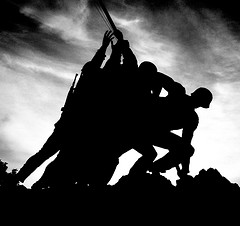
\includegraphics[width=\figwidth]{pics/8/45.png}
	\end{center}
\end{wrapfigure}
Bertha was obviously intended for use by someone far stronger than a normal human, and everyone held their breath as Twitch wobbled under the bomb’s weight. 
While he fiddled with the timer and magnetic clamps, the rest of us pondered how to get it onto the ship without blowing ourselves up. 
The other team had marked a line across the crater entrance and according to them anyone crossing it would trigger another scarab attack. 
They’d done a little testing and it seemed that it was only people that set them off; 
rocks, las bolts, bullets, and even grenades were fine so long they didn't detonate against the ship. 
Since we weren’t keen on fighting scarabs while carrying an oversized melta-bomb, this all meant that we needed to figure out a way to get Bertha onto the ship’s hull without anyone entering the crater.

Since the typical ranged melta-bomb deployment method of just throwing the thing as hard as possible wasn’t an option, the agent suggested that the last two surviving psykers could levitate the bomb across the gap. 
Sarge vetoed this on the grounds that it was an incredibly stupid idea, and was thankfully able to supply a far more reasonable solution. 
Nubby and a few recruits were sent to collect pipes and scrap metal, while Sarge regaled everyone with the tale of how we’d dealt with a similar problem involving a tentacle daemon.

By the time Twitch had the bomb ready, a long, ugly, and surprisingly-sturdy pole had been constructed, and a fulcrum was set up on the edge of the line. 
Bertha was attached to the pole with her clamps facing forward, and with the help of several trainees, we slowly pushed the rod along the fulcrum. 
It was touch and go in a few spots, especially when a seam got stuck on the brace and nearly tipped it over, but we got it across and clamped to the hull without triggering an attack or blowing ourselves to little pieces. 
Once the breaching charge was in place, our trainees set up their heavy weapons, we finalized our attack plans, and everyone shielded their eyes as Twitch hit the detonator.

Bertha was a melta-bomb, so “her” detonation wasn’t the usual flash, bang, and shockwave of high explosives. 
Instead, there was a sort of hissing-crackling sound along with intense heat, blinding light, and a whole lot of smoke, which began to roil as scarabs swarmed through it. 
We responded by opening fire with our heavy weapons, and just holding the triggers down until the smoke cleared and the scarabs stopped coming.

\begin{wrapfigure}{O}{\figwidth}
	\begin{center}
		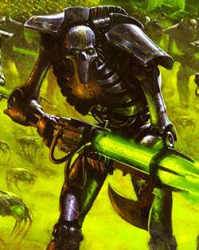
\includegraphics[width=\figwidth]{pics/8/46.png}
	\end{center}
\end{wrapfigure}
The scarabs abandoned their attack without making it through the kill-zone, and no more spider-worms (which the cogboy testily informed us were called Wraiths) appeared to back them up. 
We reloaded, formed up, and carefully made our way across the crater and through the still-glowing hole in the xenos ship’s hull.

The agent and commissar led the way, and the first thing they did after entering the ship was fall sideways out of the hole as the ship’s gravity field took over. 
We handled it a little more gracefully (after our stint on the Occurrence Border, gravity shifts didn’t really bother us anymore), and we managed to get all the trainees through without any injuries. 
The room we were in was large enough to hold our entire force and packed with all sorts of green glowy machinery. 
The cogboy was ecstatic, but didn’t see anything that looked like the teleporter, so we gathered everyone together and made our way to a large door that looked like it led towards the middle of the ship.

At our signal, our trainees began going through the now-familiar breach and clear drill. 
Charges were placed, flashes were prepped, and everyone got ready for a fight, but the enemy failed to oblige us, at least initially. 
Our boys stormed in, looking professional as all hell by the way, and found a room that seemed just as big and empty as the last one. 
Nerves jangling, we advanced across the room, and were about halfway to the next door when the enemy hit us.

Green beams lanced out of the shadows and cut down a pair of trainees while the rest of us grabbed cover. 
The hostiles that slowly stepped out of the shadows were the metal skeleton things that we’d been expecting when we’d heard the word Necron. 
After their initial advance, the xenos stood stock still, ignoring our fire and shooting green lightning from weapons that resembled spiky plasma guns. 
Their shots sliced across the room in long arcs, burning through  armor, flesh, and bone like it wasn’t even there. 
Luckily, the bulkheads and machinery that filled the room proved more resistant to the green beams, offering us a distinct advantage since the skeletal xenos didn’t appear to understand the basic concept of cover.

After the initial surprise attack we poured fire into the Necron warriors. 
There were only four of them and over thirty of us, but they were surprisingly sturdy and by the time we’d worn them down reinforcements were coming in.

\begin{wrapfigure}{O}{\figwidth}
	\begin{center}
		
\includegraphics[width=\figwidth]{pics/8/47.png}
	\end{center}
\end{wrapfigure}
Two more Necrons stepped out of the far door along with a swarm of scarabs. 
They just stood there and traded fire with us like the others had, except with the scarabs repairing them almost as fast as we did damage. 
It was damned disconcerting watching their wounds sort of flow closed and some of the recruits began to panic fire. 
Without the heavy weapons Twitch’s squad had brought down it would have been bad; 
it took a pair of our single-shot krak missiles to kill them.

As soon as the last two hostiles were dead Sarge ordered another advance, which ground to a halt a mere ten meters into the next room, when another pair Necrons entered through the far door and opened fire. 
The room was long and thin, with good cover along the sides, but no safe way to move forward. 
Our Guard instincts told us to dig in and trade fire from our superior cover, but the cogboy claimed he could sense more Necros teleporting in somewhere ahead of us, which meant that attrition tactics might not work in the long term. 
The question was whether we were killing them faster than their reinforcements were arriving, and even if we were outpacing them, whether we’d reach the teleporter before we ran out of men or ammo.

While Sarge and the other team’s were arguing over whether to risk more aggressive tactics or not, Nubby was back at the entrance to the room, sitting in the best piece of cover available. 
His attention was evenly split between taking pot-shots at the Necrons blocking forward progress, and visually inspecting the pair of dead xenos near him for anything worth pocketing. 
The little trooper nearly shit himself when both the Necons began to slowly pull themselves together and climb to their feet. 
Operating in a blind panic, Nubby sprayed one Necron with las-fire, kicked the other between the legs hard enough to knock it across the room, and ran forward screaming like a little girl. 
Only sheer luck kept him from getting hit as he ran through everyone’s line of fire.

Sarge looked back when he heard Nubby’s screams and swore. 
Back in the recently vacated room more of the Necrons were reanimating.

\begin{wrapfigure}{O}{\figwidth}
	\begin{center}
		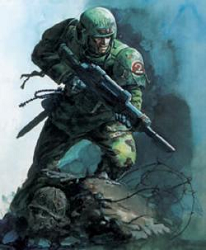
\includegraphics[width=\figwidth]{pics/8/48.png}
	\end{center}
\end{wrapfigure}
So no shit, there we were, on a crashed xenos spaceship, fighting skeletons made of living metal, and the ones behind us were getting back up. 
This was a very bad thing.

If enemy reinforcements were going to keep porting in and the ones we killed weren’t going to stay that way, there was only one real option; 
we had to push forward and destroy the teleporter before we were overwhelmed. 
Sarge gave the order to advance by squads and we all prayed to the Emperor that the xenos weren’t good at switching targets.

The trainees were not happy with that order: 
running headlong into incoming fire did NOT sound fun and the Necrons were damned scary looking. 
On the other hand, more metal skeletons were coming up from the rear, so there wasn’t anywhere else to go. 
They complained, they swore, and then they manned up and advanced; 
just like proper guardsmen.

It’s important to understand that advancing by squads is not the same as a reckless charge. 
It is a precise, difficult maneuver and it was a damned good thing that we’d drilled on it, because there were a lot of ways it could have gone horribly wrong. 
Sarge stood there and barked commands, exactly as he’d done during training, ordering one squad to throw grenades, another to lay down fire and a third to advance to a new position. 
Then, as soon as the third squad was in cover, the process would repeat; 
there wasn’t any stopping to rest or retrieve wounded, everyone had to keep moving and fighting or the whole thing would fall apart.

Some trainees died, others were badly wounded, but to a man they followed their orders and we steadily gained ground. 
It took a lot of training and discipline to pull off that sort of maneuver, and if anyone from the other team had been watching it probably would have impressed the shit out of them. 
They’d have stood there going “By the Emperor, look how coordinated and professional all those former scribes and clerics are! 
We were totally wrong about those guardsmen being a bunch of lazy incompetents, and should probably apologize”. 

Or at least they would’ve if they and their trainees hadn’t been busy holding off the re-animating Necrons behind us while we advanced.

\begin{wrapfigure}{O}{\figwidth}
	\begin{center}
		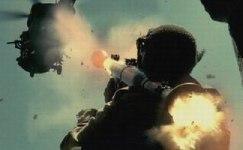
\includegraphics[width=\figwidth]{pics/8/49.png}
	\end{center}
\end{wrapfigure}
The grenade barrages before each push were our best weapon against the Necrons, since that necroderpis stuff they were made of just shrugged off most las and stubber fire. 
The hostiles were reinforcing in pairs with a few bugs repairing them, each barrage would handle the closest pair and most of our fire would focus on softening up the next two before the process repeated. 
Sarge kept everyone organized and moving, Twitch took potshots with his remaining krak missiles whenever he had a chance, and Nubby dedicated himself to making sure any downed Necrons nearby stayed that way.

The boys were starting to run out of grenades as we reached the end of the long room, but when the door opened to let a pair of hostiles though, we could see a big glowy platform thing on the far side. 
The platform looked sufficiently teleporter-like to us, and all we really needed was line of sight, so Sarge called a halt. 
Our trainees set up their heavy stubbers, we readied our few remaining krak launchers, and when the door opened again, we sighted all our weapons on the platform while a final barrage of grenades handled the advancing Necrons. 
As the door slammed back shut, we all held our breath, focused on holding our aim steady, and hoped like hell that we’d be able to get a clean shot on the teleporter the next time it opened.

When the door finally slid back open, we all fired our launchers. 
Sarge’s shot went high, sailing over the platform and blowing apart a section of wall. 
Nubby’s shot was wasted on one of the advancing Necrons, but that cleared a path for Twitch and the stubbers. 
Our last krak missile and a stream of AP rounds sailed through the door as it slammed closed again, and while we didn’t see them impact the teleporter, we sure as hell felt it.

There was a loud crackling bang, the entire ship shook, and then things got weird. 
First everything went all tingly and green colored, next Nubby spotted some of the Necron corpses sort of fading, then the walls went all wobbly, and finally there was an almighty *CLANG* and everything went back to normal.

\begin{wrapfigure}{O}{\figwidth}
	\begin{center}
		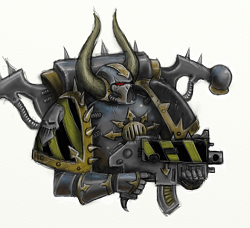
\includegraphics[width=\figwidth]{pics/8/50.png}
	\end{center}
\end{wrapfigure}
Everyone just sort of stood there looking stupid for a few seconds. 
We all expected something more to happen, like another attack or the ship exploding or a wormhole sucking us into the warp, but nothing did. 
All the hostiles had vanished, and we were just sitting there, in what seemed to be an empty ship. 
Eventually Sarge gathered everyone up and took stock.

The rearguard hadn’t had an easy time of it: 
the agent was missing an arm and unconscious, the cogboy was dead, and only the commissar was holding them together. 
We were down to under twenty effective, with a handful of wounded who might live if we didn’t run into anything else. 
On the bright side, it seemed like the fight was over; 
we’d heroically saved the day and captured a piece of highly valuable xeno-tech. 
At least it looked that way, Sarge decided to err on the side of caution and do a last sweep before we threw any parades.

The door to the teleporter room was pried open and we carefully entered. 
It didn’t have any hostiles inside and appeared to also be the ship’s the bridge. 
Half the room was taken up by the wrecked teleporter and there was what looked like an empty command chair with a few deactivated control panels, but what really caught the eye was this important looking pedestal. 
It was covered with runes that were still glowing green and had a small metal cube suspended above it in some sort of anti-grav field. 
Sarge told everyone, especially Nubby, not to touch it. 


While the rest of us poked around the bridge, Twitch made some field repairs to our least damaged vox pack. 
It didn’t take long; 
say what you will about those green beam weapons, they don’t do much collateral damage. 
The first thing Doc asked when we reached him was if WE had called for any shuttles.

The call was interrupted by the door on the far side of the bridge slamming open.

Not one, but two silver and gold giants strode into the room. 
They had huge ass bolters and far too many spikes on their armor.

\begin{wrapfigure}{O}{\figwidth}
	\begin{center}
		\includegraphics[width=\figwidth]{pics/8/51.png}
	\end{center}
\end{wrapfigure}
So no shit, there we were, standing on the bridge of an alien vessel, staring slack-jawed at a pair of Chaos Space Marines, both of whom seemed just as surprised as we were to find anyone else here. 
Everyone held very, very still and waited for someone to make the first move. 
We had them heavily outnumbered and they had us heavily outclassed. 
If this turned into a fight, it was going to be a bloodbath.
 
The staring contest stretched a little longer, and our nerve began to crack. 
Sarge carefully stepped forward and, nonchalantly as possible, asked the marines if we could help them with anything. 
This just got more blank stares and an awkward cough from Nubby, until a third figure entered the room. 
The two marines stepped aside to reveal what was obviously a Heretek, who, after a fit of buzzing and giggling, told us that yes we could indeed help them.
 
Now, most any tech-priest looks sinister, but the difference between an ugly cogboy and a full blown heretek is damned noticeable. 
Aside from all the metal tentacles, eerie lights, dripping thingies, and pointy bits, this one practically radiated insanity. 
The second you saw him it was obvious that this guy wasn’t just fucking nuts; 
he was also bolts, screws, rivets, and those metal clampy dealies you use on the prefab field buildings.
 
In a voice that seemed to be stuck looping between five different settings, and in between bouts of hysterical giggling, the Heretek demanded “the device”. 
No real clarification was needed: 
he wasn’t just staring at the cube on the pedestal, his eyes had actually extended out of his head on little mechadendrites. 
Sarge, mind racing, stalled for time by asking the crazy metal man what the cube was and why we should hand it over. 
This triggered an exasperated groan from both marines as the Heretek launched into a rambling monologue.

\begin{wrapfigure}{O}{\figwidth}
	\begin{center}
		\includegraphics[width=\figwidth]{pics/8/52.png}
	\end{center}
\end{wrapfigure}
The question had mostly been a stalling tactic while Sarge tried to figure out a way to get us out of this alive, but mixed in with all the insane chatter there were a few very important things. 
Firstly the device was a “device for devicing devices”, secondly it belonged to the Heretek because he'd “inerted the inertia and un-phased the phaser”, and finally he would make us into “meat puppets” if we didn't give it to him, now. 
We translated all this as "I am crazy, evil, easily distracted, and far more concerned with that box than you."
 
Sarge considered the situation. 
The good news was that the Heretek wanted the box so bad he might be willing to cut a deal, the bad news was that he had to have a ship of some sort in orbit and would inevitably try to kill us the moment his box was safe. 
Sarge’s assets consisted of a bunch of exhausted trainees, a paranoid, a cretin, and a still active vox link to Doc. 
He did not want to fight a pair of traitor marines, not to mention a Heretek or a bloody warp-ship; 
he wanted to live through the next few minutes and screw the other guys over before they screwed him over. 
Thinking fast he shoved Nubby forward and told him to make a deal, then waved Twitch over and tried to nonchalantly stand in front of the pedestal.
 
The negotiations would have been funny if the situation weren't so serious. 
One party was a cretinous little sneak telling outrageous lies and trying to figure out how to make a profit on this, while the other was completely insane and had no concept of what normal people wanted. 
The two marines began to look incredibly annoyed, at least insofar as a giant pile of ceramite and spikes can look anything other than murderous. 
We got the distinct impression that, if things dragged on much longer, they'd stop waiting for the Heretek's word to attack.

\begin{wrapfigure}{O}{\figwidth}
	\begin{center}
		\includegraphics[width=\figwidth]{pics/8/53.png}
	\end{center}
\end{wrapfigure}
Eventually Nubby stomped back to the rather distracted Sarge and Twitch and reported success. 
The Heretek had agreed to let us live in exchange for the box and he’d even thrown in the Necron ship on account of it being a “boring thing that attracts even boringer things”. 
That was about the best deal we could expect to get and Nubby had bought just enough time to finish the preparations, so Sarge accepted and stepped away from the pedestal, poker face firmly in place.
 
In a loud, clear voice that just happened to be directed towards the vox unit, Sarge announced that we’d be withdrawing to the room behind us. 
We’d be back there sitting still, while the Heretek and two chaos marines with bolters went up to their shuttle, the one on the roof, that would take them to their ship, the one that was in orbit. 
We would stay down here and do absolutely nothing to SABOTAGE THEIR SHUTTLE or INTERCEPT THEIR SHIP.
 
Sarge’s acting skills may have left something to be desired, but the Heretek didn’t seem to notice and the marines didn’t seem to care. 
He also somehow managed to fool the commissar since the idiot accused us all of heresy and might have caused serious trouble if Nubby hadn’t come up behind him and kicked him very firmly between the legs. 
The second kick was probably uncalled for, and the third definitely was, but no one said anything: 
we were all busy slowly backing out of the room while watching the marines.
 
Our retreat had taken us almost all the way to the door when the Heretek told us to stop. 
Hearts racing, we all froze and watched as his mechadendrites shot out and ripped the cleverly concealed explosives off the box and pedestal. 
The crazy cogboy made a comment about not needing any more explosives, thanked us for the thought, and tossed the detpacks to Twitch, who nearly fumbled them in his surprise. 

 
We all kept backing up and tried not to let our disappointment show. 
This was apparently not a problem we could solve with detpacks. 
At least not immediately.

\begin{wrapfigure}{O}{\figwidth}
	\begin{center}
		\includegraphics[width=\figwidth]{pics/8/54.png}
	\end{center}
\end{wrapfigure}
Once the door was closed and we were sure no angry traitor marines were coming after us, we all turned and ran for the exit. 
Except for the commissar that is: 
he was being dragged between two other trainees. 
As we ran, Twitch got the vox-unit patched into our comms, and Sarge asked Doc if he’d gotten all that. 
The heretics had to be stopped before they got their shuttle into the air and then their ship needed to be taken out before it just nuked us from orbit.
 
Back on the surface, Doc was looking at a very big and sturdy looking shuttle, in rather petulant voice he told Sarge that “Damn it man, I’m a doctor, not a demolitions expert!” Twitch unhelpfully reminded everyone that he was a demolitions expert, but had been forced to trade places and hike all the way down here. 
Sarge told him to be quiet unless he had something useful to say.
 
Doc was in a bind. 
The rest of us were coming up through the bunker as quickly as possible, but the heretics would probably reach their shuttle first. 
He had to figure out a way to cripple their shuttle or delay the enemy long enough for the rest of us to arrive. 
He didn’t have much to work with: 
the Heretek’s shuttle had destroyed our fliers as it landed, and the only anti-armor munitions that hadn’t been in them had been used in breaching the Necron ship. 
All Doc had was a handful of wounded troopers, a few lasguns and chainswords, a semi-conscious Cutter, and a crate of medical supplies. 


A BIG crate of medical supplies. 


A big crate of MILITARY-GRADE medical supplies.
 
Thinking fast and abandoning all medical ethics, Doc started digging into the crate and planning one hell of an ambush.

\begin{wrapfigure}{O}{\figwidth}
	\begin{center}
		\includegraphics[width=\figwidth]{pics/8/55.png}
	\end{center}
\end{wrapfigure}
While Doc was working on the shuttle problem, Sarge was trying to have a vox conversation while running. 
He’d managed to contact the Rogue Trader who’d helped us set up the whole kidnapping thing, but he was running into problems. 
The Trader had maneuvered his ship to our general side of the planet, but while he’d have been happy to lend us some orbital fire-support in exchange for a bit of Inquisitorial good-will, getting in a fight with another warp-ship was an entirely different matter. 
To put it bluntly, he wasn’t going to risk his ship, even on an ambush, for a mere bunch of Inquisitorial henchmen. 
He needed some sort of motivation.

Sarge didn’t have time, or breath, to spare arguing with the Trader. 
We needed the man’s help: 
there were no other ships close enough, or well-armed enough, to stop the Heretek’s vessel, so Sarge cut a deal. 
It wasn’t a smart deal, in fact there was a very real chance that Inquisition would have him killed for even considering making it, but it was the only way he could see out of the current situation. 
Sarge offered the only really valuable thing he had: 
one slightly used Necron ship.

You better believe that caught the Trader’s attention.

Sarge gave what evidence he could that the ship was actually there and greed did the rest. 
The Trader said he’d handle whatever vessel the Heretek was using or damn well die trying; 
the prize was worth it.

That done with, we laid on the speed. 
It was a clear run up through the bunker, since all the cultists were either dead or fleeing, and we all ran flat out. 
There was no real plan, it was just going to be a matter of getting to the roof and hitting them in the rear while Doc held their attention. 
No finesse, no trickery, just the biggest sucker punch we could manage.

We either made amazing time or the Heretek had taken a while getting the box off the pedestal, because we got there right as Doc’s ambush hit them.

Let me tell you, that was really something to see. 
Hell, we were so busy watching that we almost forgot to fire our weapons.

\begin{wrapfigure}{O}{\figwidth}
	\begin{center}
		\includegraphics[width=\figwidth]{pics/8/56.png}
	\end{center}
\end{wrapfigure}
Some of you might know what Slaught and Frenzon are, but if you don’t, imagine the fastest, meanest, angriest bastard you’ve ever seen. 
Now give him an immunity to pain, rabies, and slight brain damage. 
That’s what a dose does to a normal person. 
What a double dose cut with stimms did to Cutter and his boys was just ridiculous.

Doc had got them positioned, timed their injections, and let them loose at just about the perfect moment. 
A bunch of half-dead mudfeet turned into enraged murder-machines about three meters from the Heretek and his marines, right as they were getting off the hover-thingies that they rode up out of the crater on. 
The fight was too fast to follow, we just did had to aim for the enemy and hope our shots didn’t hit any of Cutter’s boys.

I’d like to say it was a heroic and complex battle, but really we just poured fire into the two traitor marines until the sheer mass of it overwhelmed them. 
Sure, they had superhuman strength, hundreds of years of battle experience, and whatever daemonic powers their dark masters had granted them, but as we say in the Guard “Quantity has a quality all its own”. 
Las and stub rounds, only a minor threat individually, pounded into them in a continuous torrent that even they couldn’t ignore. 
Simultaneously, the chem-powered chainsword strikes of our berserkers tore deep rents in their power-armor and kept them from bringing their bolters to bear on the rest of us. 
It wasn’t all one-sided of course, multiple trainees fell to sprays of unaimed bolt rounds, and even without proper melee weapons, the traitor-marines were capable of dealing horrible damage to the berserkers attacking them. 
Unfortunately for them, “horrible” isn’t the same as “incapacitating” for someone hopped up on combat-chems: 
even as our berserkers bled out, they pressed their attack, and forced the two space marines to give ground which they didn’t actually have. 
First one marine, then the other, was pressed backwards and over the edge of the crater. 
They pancaked on the crashed ship with a sort of crunchy splatting sound.

The Heretek didn’t go down as easily as his bodyguards though. 
He had some sort of shield which blocked all of our fire, and quickly dismembered everyone who got into melee range until just the king berserker himself was left. 
The rest of us desperately poured fire into the Heretek’s shield in an attempt to burn through it, while Cutter duked it out one-on-one with the crazy cogboy.

\begin{wrapfigure}{O}{\figwidth}
	\begin{center}
		\includegraphics[width=\figwidth]{pics/8/57.png}
	\end{center}
\end{wrapfigure}
Cutter was being kept on his feet by a cocktail of drugs that would probably kill him the moment they ran out; 
his time was measured in seconds. 
Seconds were all he needed though.

He didn’t bother with dodging, parrying, or any sissy stuff like that: 
all he cared about was doing as much damage as possible. 
Mechadendrites ripped off chunks of flesh, a sparking weapon nailed him in the legs, and some sort of injector just barely missed his heart, but Cutter ignored these trivialities. 
He lodged his faithful chainsword firmly in the Heretek’s chest and wrenched it upwards with berserk strength.

The deranged cogboy screamed and flailed as he was bisected, writhing so violently that pieces started flying off, one of which landed within Nubby’s reach and was promptly pocketed. 
As the chain-blade reached the base of the Heretek’s neck, his screaming finally coalesced into one word repeated in a dozen voices: 
“Burn”. 


There was a second of unnatural silence, followed by a rising humming sound, and then the Heretek exploded into a fireball that engulfed both him and his attacker. 
Cutter laughed as he burned.

All in all, there were worse ways to go.

\begin{wrapfigure}{O}{\figwidth}
	\begin{center}
		\includegraphics[width=\figwidth]{pics/8/58.png}
	\end{center}
\end{wrapfigure}
There wasn’t time to stand around in shock or mourn Cutter’s death. 
A few seconds after the Heretek’s self-immolation, a massive energy beam hit the nearby shuttle, and we realized the crazy bastard had called for an orbital bombardment.

We grabbed what wounded we could and ran back into the cult’s bunker; 
it was the only option we could see. 
We sprinted through hallways and down stairs with titanic explosions filling our ears and uncomfortable dampness filling our pants. 
One by one the unfit and the badly wounded fell behind, as did the bow-legged commissar, and those who fell behind, were left behind.

Nubby led the way on his augmetic legs while we all followed and hoped his cowardly instincts would lead us to safety. 
We ran through the wreckage of our battles and, just barely ahead of a titanic wave of heat, we scrambled into the Necron ship. 
None of us stopped there though, we kept going until we reached the bridge and then held our breath as the entire ship began to shake.

The shaking went on for a while, but there was no sudden burst of heat and light. 
Eventually, it all went quiet. 
Our heart rates slowed as we realized that, somehow, we’d survived the bombardment. 
Doc started crying.

\begin{wrapfigure}{O}{\figwidth}
	\begin{center}
		\includegraphics[width=\figwidth]{pics/8/59.png}
	\end{center}
\end{wrapfigure}
We sat in that ship for what felt like days. 
The hole we’d melted in the hull was clogged with debris, so there was nothing to do but wait and hope someone came looking for us.

There were fifteen of us all together: 
us four guardsmen, the wounded agent we’d left in the ship, eight of our trainees, and two more from the other team. 
As usual, Sarge took command of the whole show and got everyone up and moving. 
Doc was hauled to his feet and told that living wounded  took priority over dead heroes. 
Sarge promised that he’d be allowed to sit around feeling guilty about Cutter and all the trainees he’d drugged once we’d been rescued. 
Twitch and Nubby had already started collecting what food and water had been in people's packs, so they were put in charge of rationing after a stern reminder that everyone got a portion, not just us and the trainees they liked. 
Supply-wise we had a few weapons, a little bit of food and water, a medkit, and one Necron box thing that Nubby had snagged. 
Not much useful stuff, but at least the creepy-ass green glow the ship emitted meant we weren’t going to run out of light.

Our time down there wasn’t as bad as you’d think. 
Everyone was so tired that we slept through most of it, and our short periods of wakefulness were occupied with the usual Guard pastimes of poker, pointless tasks thought up by your Sergeant to keep you out of trouble, and idle vandalism. 
The most exciting moment of the whole experience was when Nubby and Twitch emptied the thermite out of a few anti-armor rounds, and used it to write their names on a few of the bulkheads.

Long before food and water became a problem, our boredom was interrupted by a titanic groaning sound and some disconcerting fluctuations in the ship’s gravity. 
We all wandered down to the debris-clogged hole we’d entered through, and watched as the rock and rebar began to shift, and then float away. 
As the last of the debris rose away from the opening, there was a sudden lurch, and the entire crater-wall began sliding past the breach. 
A few seconds later we were nearly blinded as the Necron ship rose into full sunlight.

The ship’s ascent slowed to a stop as it reached the top of the crater, revealing a blasted hellscape where the cult’s facility had been. 
All things considered, we thought it looked absolutely beautiful, and stood there basking in the sunlight and thanking the Emperor for our rescue, until a broad-shouldered man in a tricorn hat and a gaudy coat climbed up onto the edge of the hole and told us to get the hell off his ship. 
Apparently, he was a busy man with things to do and xeno-tech experts to see.

\begin{wrapfigure}{O}{\figwidth}
	\begin{center}
		\includegraphics[width=\figwidth]{pics/8/60.png}
	\end{center}
\end{wrapfigure}
The Trader was nice enough to call us a ride before he tractored up the Necron ship and headed out-system at his vessel’s top speed. 
He seemed to think that we might change our minds now that we were no longer being bombarded and wanted to be far away before any Inquisition fleets showed up.

A few PDF fliers picked us all up and dropped us off at our training base, where the Administrator and Surgeon were waiting on the pad. 
Doc handed the one-armed agent and the injured trainees over to Surgeon while the rest of explained the whole bloody mess to the Admin and asked him to get started on a report for the Interrogator. 
Then we went and got drunk. 
Very, very drunk.

Training was over after that; 
the few recruits that had survived were officially Inquisitorial agents as far as we were concerned. 
We all just sort of lounged around, reminisced about Cutter, and speculated about what the Interrogator and Oak would say when they saw how many trainees we had left. 
The agent and his trainees stayed with us, since aside from the psyker chick who had been badly hurt during the investigation, he was all that was left of his team. 
He wasn’t that bad of a guy really, once you got to know him. 
A bit of a downer though.

Eventually the Interrogator arrived and we gave our report: 
Eight recruits trained and ready for service, plus a handful of washouts and two from the other team. 
Also, as a side note, we destroyed an evil cult, found and secured a Necron ship, got into a fight with a Heretek, traded said Necron ship to a Rogue Trader, and now all we have is this Necron box thing and everyone is dead. 
That got the aloof bastard to pay attention.

\begin{wrapfigure}{O}{\figwidth}
	\begin{center}
		\includegraphics[width=\figwidth]{pics/8/61.png}
	\end{center}
\end{wrapfigure}
It took a lot of explaining, mostly by Sarge and the agent. 
The whole story was gone through, from start to finish, sparing no detail. 
The Interrogator didn’t judge or lecture, he simply made sure he had all the facts straight then put them all into a neat report. 
In the end he decided this was above his paygrade, took our recruits, and sent us all back to Oak with the little Necron box. 
The agent and his psyker companion were told to stay on the planet until they’d fully recovered from their injuries.

The trip home was about as normal as warp travel gets. 
Nothing particularly interesting happened, unless you count Twitch nearly killing a naval rating who was cleaning the air ducts. 
Or Doc getting accused of stealing from the ship’s medbay while observing the head Medicae’s surgical procedures. 
Or Sarge catching Nubby selling several crates of medical narcotics that he’d “found somewhere” to the crew. 
Anyway, we survived the trip, and since the Interrogator’s report had been sent ahead of us, an escort was waiting for us when we docked with Oak’s ship. 
Our entire group was marched to the Inquisitor’s office and our story was gone over yet again.

To our surprise Oak was not angry, not even when we mentioned giving the Rogue Trader the Necron ship. 
He shrugged that off as something to be dealt with later, if the Necrons didn’t deal with it themselves, and focused his attention on the little box Nubby had retrieved instead. 
It seemed inordinately important to him: 
he asked us a lot of questions about what the Heretek had said about it and was a little annoyed when we couldn’t give him anything besides insane babble. 
In the end he took the box, told us we all did exceptionally well, and instructed us not to talk to anyone about it, even inside the Inquisition, without his direct permission. 
Then we went and got drunk again.

\begin{wrapfigure}{O}{\figwidth}
	\begin{center}
		\includegraphics[width=\figwidth]{pics/8/62.png}
	\end{center}
\end{wrapfigure}
Cutter’s funeral was a pretty big deal, and we got everyone we could to come to it. 
In addition to the other guardsmen from the old regiment, there were a few cogboys, including Jim and Hannah, the hospitaller and a few other sisters, the old adept lady and finally, to our considerable surprise, the Rupert and Alfred.

It was a hell of a party. 
Both stories and beer flowed freely, but the real crowning moment was when the Rupert brought out his death offering. 
Emperor knows where he, or more likely Alfred, got it, but it was one of those orky chainswords; 
a perfect match for Cutter’s. 
It floored us all, even Sarge was crying as we put it in the plasma chamber with everything else. 
It was a damned fine send-off; 
we did him proud.

Days later, after the beer had run dry and the hangovers had cleared, we got another visit from the Rupert and Alfred. 
He told us, in his own unique way, that he’d asked Oak to transfer us to his retinue, but the Inquisitor had declined. 
Apparently, Oak thought he might need our services in the future, but as a favor to his former student, he’d consider sending our next Interrogator to work with the Rupert.

It took a while for the situation to sink in, but it did eventually. 
Sarge thanked the Rupert and said he’d be happy to serve alongside him again and hoped the Interrogator we’d officially be under wasn’t a complete tit.

He turned out to be a complete tit.
